\documentclass[stu,12pt,floatsintext]{apa7}
\usepackage[american]{babel}
\usepackage{csquotes}
\usepackage[style=apa,sortcites=true,sorting=nyt,backend=biber]{biblatex}
\DeclareLanguageMapping{american}{american-apa}
\usepackage[T1]{fontenc}
\usepackage{mathptmx}
\usepackage{graphicx}
\usepackage{array}
\usepackage{multirow}
\usepackage[labelsep=newline,labelfont=bf]{caption}
\usepackage{multicol}
\usepackage{makecell}
\usepackage{amsmath}
\usepackage{float}
\usepackage{setspace}

\addbibresource{references.bib}

\renewcommand{\enumerate}{\APAenumerate}
\renewcommand{\itemize}{\APAitemize}
\let\oldsection\section
\renewcommand{\section}{\newpage\oldsection}

\DeclareMathOperator*{\argmin}{arg\,min}
\DeclareMathOperator*{\argmax}{arg\,max}

\title{Customer Satisfaction Based On Written Reviews on E-Commerce Websites:\\
An Analysis Of Various Machine Learning Models}
\author{Shrey Agarwal, Joseph Chang, Ibrahim Khalid, Justin Wang}
\authorsaffiliations{{Department of Applied Data Science, San Jose State University}}
\course{DATA 270: Data Analytics Processes}
\professor{Dr. Linsey Pang}
\duedate{May 6, 2024}

\abstract{Product reviews are widely used in e-commerce as a way for users to voice their opinions about products and services. By categorizing reviews as positive and negative, companies may be able to obtain insights on how to improve their products. With a diverse range of products and categories, the Amazon Product Reviews dataset allows researchers to conduct a detailed analysis and develop machine learning models to extract meaningful insights and identify useful trends in the e-commerce industry. Major attributes include user reviews and ratings that accurately capture and represent users' opinions. The primary objective is to measure sentiments expressed in the reviews by using a variety of supervised learning techniques including Logistic Regression, Naive Bayes, Support Vector Machines (SVM), and XGBoost. This involves training on various datasets across categories in order to accurately capture the model’s effectiveness, before comparing it against a sample testing set. Evaluation metrics include measuring the accuracy, precision and recall, as well as constructing confusion matrices, in order to properly compare each model’s performance. Project deliverables include all source code for the models, demonstrations, presentations, and a final completed report. The intent is to present an accuracy metric for sentiment analysis and compare with actual users' attitudes. Other factors such as time to train and cost of product will also be taken into account when comparing the models. Ultimately, this project aims to emphasize the importance of Amazon’s product reviews as a potential resource for scientists and scholars developing research on recommender systems, current market trends, and human psychology. The conclusion will summarize the findings that can help with future decision-making processes and provide a more informed user experience.}

\keywords{Sentiment Analysis, Recommendation System, e-commerce, Amazon product reviews}

\begin{document}
\maketitle
In an increasingly technological society, people have come to rely on computers and technology as a tool for various aspects of life, including shopping. Notably, the online shopping industry has changed significantly over the past decade, where product reviews have emerged as an important factor in purchasing decisions and current market trends. Among the many e-commerce platforms such as Ebay or Flipkart, Amazon has become popular and widely utilized for product reviews, spanning thousands of categories. As customers are consistently seeking the optimal quality at the most reasonable price, evaluations from other consumers is important and needed because it can be the most dependable resource to make a purchase and meet their demands \parencite{verma2022sentiment}. Organizations can also analyze the reviews on their products to better gauge customer satisfaction. In particular, they can filter out reviews that are positive or negative and make decisions to further improve their business. 

\subsection{Executive Summary}
A fundamental aspect and targeted problem of this project is Sentiment Analysis, which is defined as the process of analyzing text to determine the sentiment or opinion that the text will convey \parencite{saridena2023sentiment}. Reviews are sometimes not collected in industry settings, so the categorization of reviews serves as valuable feedback, allowing for the extraction of meaningful insights and identifying areas for improvement. By exploring the Amazon’s Product Reviews dataset provided by \textcite{ni2019justifying_dataset}, which offers a rich and comprehensive exploration of user preferences and sentiments in this technology-driven era, the goal of this research is to create a system that can classify unlabeled reviews into one of the following categories: negative, neutral, or positive. 

\subsubsection{Planned Project Approach and Methods}
The dataset that is being used contains a collection of Amazon Product Reviews by category. To make this dataset more usable, each review must first be labeled with a sentiment. On top of this, the data must be downsampled due to the sentiments being skewed in favor of positive reviews. To achieve optimal representation and results, it is crucial to eliminate features that may negatively impact the models performance. Additionally, various Natural Language Processing (NLP) techniques will be applied to the text in order to allow the machine learning models to process and understand each review; this includes removing filler words, removing punctuation, standardizing the letter case, and finally vectorizing or tokenizing the sentences. On top of the standard preprocessing, the research will experiment with stemming and lemmatization on the sentences in an attempt to identify which methods can more efficiently categorize the data the best. The plan is to use these preprocessed sentences to train traditional classification machine learning algorithms and models such as decision trees, support vector machines, K-nearest-neighbor, and logistic regression. Then, based on the results, we plan to perform hyperparameter tuning using tools such as RandomizedSearchCV or GridSearchCV, as well as adding more restrictions to our preprocessing methods.

\subsubsection{Expected project contributions and applications}
This methodology has many useful applications, not only for businesses gauging public and consumer interest regarding its services and products, but also to various academic and research institutes. Scholars and scientists can leverage the developed insights to develop their own recommender systems that can predict user’ preferences and potential purchases based on reviews. In addition, psychologists can gain valuable insights for basic human behavior, interactions, and preferences while understanding and analyzing current trends. Before making a decision, customers can see the reviews of previous customers to make an informed decision. 

Ultimately, this research will assess whether integrating these insights can lead to a richer, more positive experience for the user and increased customer satisfaction. 

\subsection{Project Requirements}
\subsubsection{Functional Requirements}
The data must contain high quality samples as well as varying levels of language and words in order to reflect real reviews made by people. Most importantly, the data must contain sentiment labels, or features that allow the imputation of sentiments such as ratings. Due to these requirements, the Amazon Product Review dataset, which contains a massive amount of reviews and ratings, is a sufficient dataset. This provides a diverse spectrum of data improving the model’s learning capability. With this data, we are able to use the ratings (numbered between 1 and 5) to manually label each review with sentiments based on the following conditions: 1-2 as negative, 3 as neutral, and 4-5 as positive. This method, however, is not perfect in the fringe case where the reviewer rates a product positively but their review says otherwise or vice versa. 

The hardware required for functionally training the models can either be a GPU enabled system with sufficiently high RAM or a cloud enabled coding platform such as Google Colab. The essential Python libraries include Regex and NLTK for sentence preprocessing, as well as scikit-learn for machine learning, in addition to the standard data handling libraries such as pandas and numpy.


\subsubsection{Machine Learning Model Requirements}
A variety of machine learning models will be used and evaluated with performance metrics such as accuracy, precision, recall, and confusion matrices. In addition to the models, users will need to be familiar with the following sentence preprocessing methods: character removal, stemming and lemmatization, tokenization and vectorization. Training the models will require us to perform hyperparameter tuning via various cross validation methods.

The plan is to use the following machine learning techniques:

\paragraph{Decision Trees} are a machine learning model that can be used for classification. According to \textcite{ibm2024decisiontree}, decision tree learning uses a divide and conquer strategy to identify split points in the tree, eventually classifying all of the data. To enhance their performance, bagging techniques (Random Forest) or boosting techniques (XGBoost) are used.

\paragraph{Logistic Regression} is a classification algorithm that utilizes supervised learning techniques to predict the probability of the data falling under a specific class. Due to its simplistic nature, this makes it a good candidate for use as a baseline measure.

\paragraph{Naive Bayes} is a probabilistic technique based on Bayes' Theorem. It is considered a generative learning algorithm, which means that it models the distribution of inputs of a given class rather than learning which features are the most important for each class. 

\paragraph{Support Vector Machines} are particularly powerful when it comes to text categorization and classification due to the high input dimensionality of textual data \parencite{joachims1998svm}. This makes it a good candidate for sentiment analysis. Since the data is classified into 3 levels, a one vs many approach to the model will be employed.

\subsubsection{Data Requirements}
The Amazon Product Review dataset consists of 233.1 million reviews, contains a large variety of product categories, and was collected between May 1996 to October 2018. There are many features, but the most important ones include the overall rating (out of 5), a binary indicator of whether or not the review is verified, the review text, and its summary. Note that the reviews are not labeled with a sentiment, so labeling them based on the rating is needed. Verified reviews inform whether the customer leaving the review actually used the product or not, and whether they paid the full price of the product \parencite{amazon2024help_verified}.

Due to the nature of online reviews and the biases that a customer possesses while leaving a review, the distribution of the ratings follows a J-shaped distribution \parencite{hu2009overcoming}. See Figure \ref{fig:j_shaped_distribution} for the shape of the dataset. To mitigate this undersampling and minimize this bias, removing a certain number of 5-star reviews by random can be employed. 

\begin{figure}
    \centering
    \caption{Distribution of product review ratings and sentiments}
    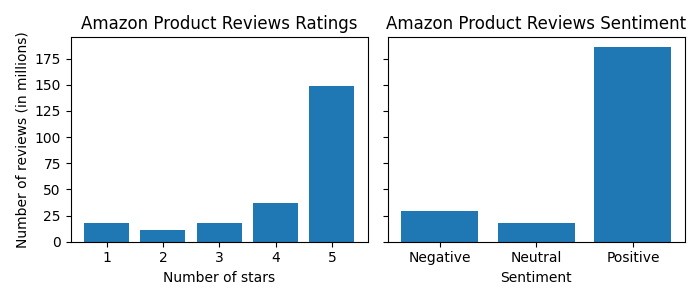
\includegraphics[width=0.9\linewidth]{images/results/all_review_distribution.png}
    \label{fig:j_shaped_distribution}
\end{figure}


\subsection{Project Deliverables}
This project consists of many deliverables in the form of documents and source codes. 

\subsubsection{Documents}
The documents of this project are as follows:

\begin{itemize}
    \item Abstract report and presentation.
    \item Chapter 1 report and presentation covering the introduction to the project as a whole. 
    \item Chapter 2 report and presentation covering data and project management plan.
    \item Chapter 3 report and presentation covering data engineering.
    \item Chapter 4 report and presentation covering model development.
    \item An individual report on Support Vector Machines.
    \item An individual report on Logistic Regression.
    \item An individual report on Naive Bayes.
    \item An individual report on XGBoost.
    \item A final report document with all chapters included.
    \item Code documentation detailing how to train and run the models.
\end{itemize}
Note: each subsequent report extends the previous report.
\subsubsection{Source Codes}
\begin{itemize}
    \item System requirements file for python virtual environment.
    \item Jupyter Notebook files containing code for ETL, preprocessing, and model training.
    \item Jupyter Notebook files used for exploring the dataset.
    \item Github repository link to the project.
\end{itemize}

\subsection{Technology and Solution Survey}
There are many current different technologies and solutions, along with this problem statement, in which sentiment analysis can provide meaningful insights. Before a model can classify the sentiment, the data must be posed in a representation that is easy for the model to understand. This is where Natural Language Processing (NLP) is used to analyze and preprocess the data. In various research, Dr. Sindhura points out that the Natural Language Toolkit (NLTK) library provides a repository for performing various natural language processing tasks. It provides access to the set of stopwords which add little to no value in a sentence, and to the WordNetLemmatizer package which performs Lemmatization \parencite{sindhura2023sentiment}.  

The first several steps focus on feature manipulation and changes to representation of sentences in reviews as part of the preprocessing phase. Pandas is used to perform a wide variety of feature adjustment and removal to a dataset. Using this library, extraneous features that don’t offer value for the model can be removed, and the mapping to assign a numerical value which will define positive, negative, or neutral sentiment will be performed. The reviewText column contains text of each review which is where the bulk of the information is located and will be used for classifying the sentiment. It is crucial to remove any extraneous symbols such as punctuation, including hyphens, question marks, periods, exclamation, or other symbols that will impact the model performance. This can be done through regular expressions to remove any extraneous characters. It is likely for the reviews to have a high frequency of stopwords. Since it has been established that stopwords add no value, all stopwords from reviewText through subsequent preprocessing steps will be removed. In a similar Amazon driven sentiment analysis project, high frequency of stopwords are removed from the dataset through the course of several preprocessing steps. Lemmatization is then performed using the WordLemmatizer package in the NLTK library. This is where the words in the text are converted into their simpler base format. The words need to then be converted into some numeric representation that the model will understand. The sklearn CountVectorizer package is utilized to create a word count vector and perform tokenization. To classify the sentiment of the reviews, Regression and Naive Bayes models are utilized. The two models are compared on a performance basis based on evaluation metrics like accuracy score, precision, and recall. From the accuracy score point of view, the performance is relatively the same. The logistic regression model had an accuracy of 89\% using a bag-of-words and 88\% using TF-IDF, as opposed to Naive Bayes which had an accuracy of about 88.9\% and 88.8\% respectively \parencite{jain2020amazon}. It can be seen that there is a minor difference in the accuracy. Hence, training both models to see which one would have a better performance will be crucial.   

It is also possible to use ensemble techniques to classify the sentiment of Amazon reviews. In a similar research project performed by \textcite{sadhasivam2019sentiment}, they combined Naive Bayes and SVM (Support Vector Machine). This created an ensemble algorithm which further improved the outcomes. The accuracy of the ensemble technique was around 73\% for positive classes and 78\% for the negative classes. For the Naive Bayes model itself, the overall accuracy was around 32\% and 37\% for the negative classes. For the SVM itself, the accuracy was around 27\% for positive classes and 37\% for negative classes. Based on the results, the ensemble algorithm clearly had better performance over the other 2 options. Hence, ensemble techniques and models such as Random Forest and XGBoost will also be utilized to obtain better performance. 

Based on the survey of these papers, our group has made the decision to utilize Natural Language Processing (NLP) techniques, specifically from the NLTK and scikit-learn libraries, to preprocess the data. This preprocessing is essential for the training of our models, as reviews often contain misspelled words and unnecessary characters which may interfere with our models’ ability to learn and capture trends. In addition, we will train multiple algorithms like SVM, decision trees, logistic regression, and Naive Bayes and evaluate its results to determine which method performed the best, as well as consider ensemble methods (bagging and boosting) due to their potential boost in performance.


\subsection{Literature Survey of Existing Research}
In the exploration of the Amazon Product Reviews dataset, this research will compare various machine learning algorithms and techniques from training and testing sets. This includes supervised learning, which is a prominent field in computer science that utilizes data to construct computational models for predictions and decision-making \parencite{saridena2023sentiment}. Specifically, the focus lies within binary classification problems, which is a subset of supervised learning, where the label's outcomes are limited to only 0 or 1 \parencite{saridena2023sentiment}. Depending on the context, 0 signifies a negatively-reviewed sentiment, while 1 represents a positively-reviewed sentiment. The neural network's output, denoted as $\gamma_\epsilon$ (0,1), is a function of the features, and it predicts whether an example will fall in category 1 if $\gamma_\epsilon > 0.5$, or in category 0 if $\gamma_\epsilon < 0.5$. Sigmoid activation functions, or ``softmax'', are usually applied in these binary classification problems to ensure the output of the model always is either 0 and 1. This method enhances the model's predictions, making it effective for predicting sentiments in product reviews \parencite{saridena2023sentiment}.

\textcite{zhu2018adversarial} worked on an adversarial review generation model on the same dataset as in this research. In that study, they recorded a precision score of 0.3 for predicting negative reviews without downsampling, whereas there was a precision score of 0.96 for predicting positive reviews in the same model and data configuration. To mitigate this issue, they employed down sampling the positive reviews.

\textcite{verma2022sentiment} trained and compared Multinomial Naive Bayes (MNB), Logistic Regression, and a LSTM network on a dataset containing 400,000 reviews. After performing various preprocessing techniques and converting the sentences into vectors using a bag of words approach and a TF-IDF approach, Verma concluded that Logistic Regression performed the best, with an accuracy of 95.63\% using a TF-IDF vectorizer, as opposed to MNB scoring a maximum of 91.84\% with bag of words and LSTM with 94.40\% with Word2Vector Embedding.

\section{Data and Project Management Plan}

\subsection{Data Management Plan}
\subsubsection{Data collection approaches}
The data collection method used in this project is downloaded from the Amazon Product Review dataset provided and obtained by University of California, San Diego in the form of a GZIP-compressed JSON file. This dataset contains a total of 233.1 million reviews collected between May 1996 and October 2018 across 29 product categories. In order to reduce computation time and cost, we have chosen the following 6 categories: `Musical Instruments', `Arts, Crafts, and Sewing', `All Beauty', `Amazon Fashion', `Appliances', and `Software'. The categories will be combined into a master dataset as a CSV file. To further cut down on time and cost, we will be using the 5-core subsets. According to \textcite{ni2019justifying_dataset}, the 5-core subset consists of reviews of items that have at least 5 reviews and reviews from users who have submitted 5 reviews. This new combined dataset contains 749,404 entries.

Since this dataset is publicly available, there are no specific data usage mechanisms we need to consider in terms of licences and usage rights. Regarding its storage, management, and processing needs, we have detailed it in the following sections.

\subsubsection{Storage and Management Methods}
Given the substantial size of the Amazon Product Review dataset, which can reach up to a maximum of 34 GB, we have chosen to store it as a GZIP-compressed JSON file. This will allow and enable us to manage data effectively and efficiently while conserving space for storage. For the chosen subset, we'll employ Git-LFS (Large File Storage) for version control and a collaborative workspace. This approach guarantees dataset consistency across team members and devices.

\subsubsection{Data Processing Needs}
We will merge the category-specific datasets into a unified dataframe for a more comprehensive analysis that we can use to extract meaningful insights. After creating the master dataset, it is evident that extensive data cleaning and preprocessing is required before analysis, see Table \ref{tab:combined-null}. The processing steps will include dropping unnecessary and redundant columns, filtering out null entries, and assigning sentiments based on the `overall' score. Since the columns we are interested in have a very small number of null values, we can justify filtering all rows with nulls. The next step will be to perform the appropriate text manipulations on the `reviewText' and `summary' columns by tokenizing, stemming, or lemmatizing. Lastly we will downsample the positive sentiments to remove the J-shaped class imbalance.

\begin{table}[!htb]
    \centering
    \caption{Null columns and column uses}
    \begin{tabular}{ccc}
        \hline
        Column name & Number of null & Usage \\ 
        \hline
        overall & 0 &calculate sentiment\\
        verified & 0 &keep\\
        reviewTime & 0 &discard\\
        reviewerID & 0 &discard\\
        asin & 0 &discard\\
        style & 380,030 &discard\\
        reviewerName & 122 &discard\\
        reviewText & 371 &keep, remove nulls\\
        summary & 192 &keep, remove nulls\\
        unixReviewTime & 0 &discard\\
        vote & 636,787 &discard\\
        image & 733,623 &discard\\ 
        \hline
    \end{tabular}
    \label{tab:combined-null}
\end{table}

The approach that we have chosen is to utilize Git-LFS for version storage. This will ensure the dataset is managed efficiently that will allow easy-to-use collaboration among the team members. In order to conduct data analysis, we will employ  a variety of Python libraries like Pandas, Numpy, Matplotlib to read in the compressed JSON file so that it is a structured dataframe, then facilitate exploratory data analysis (EDA), and achieve the tasks that the model will produce. 

As the project continues, we will actively refine our data processing pipeline as needed and leverage the advanced techniques learned in class lectures throughout the semester or through the internet findings on our own about the Amazon Product Review dataset. In working simultaneously with the class topics, the goal of this project is to extract meaningful conclusions so that our research objectives are addressed clearly and effectively and also the results can make an impact to audiences of the paper.


\subsection{Project Development Methodology}
Our project will follow the methodology of Cross-Industry Standard Process for Data Mining (CRISP-DM), see Figure \ref{fig:crispdm}. This is a standard process commonly used in the data analytics/mining scene and is comprised of the six main steps outlined below: 

\begin{figure}[!htb]
    \centering
    \caption{Cross-industry standard process for data mining}
    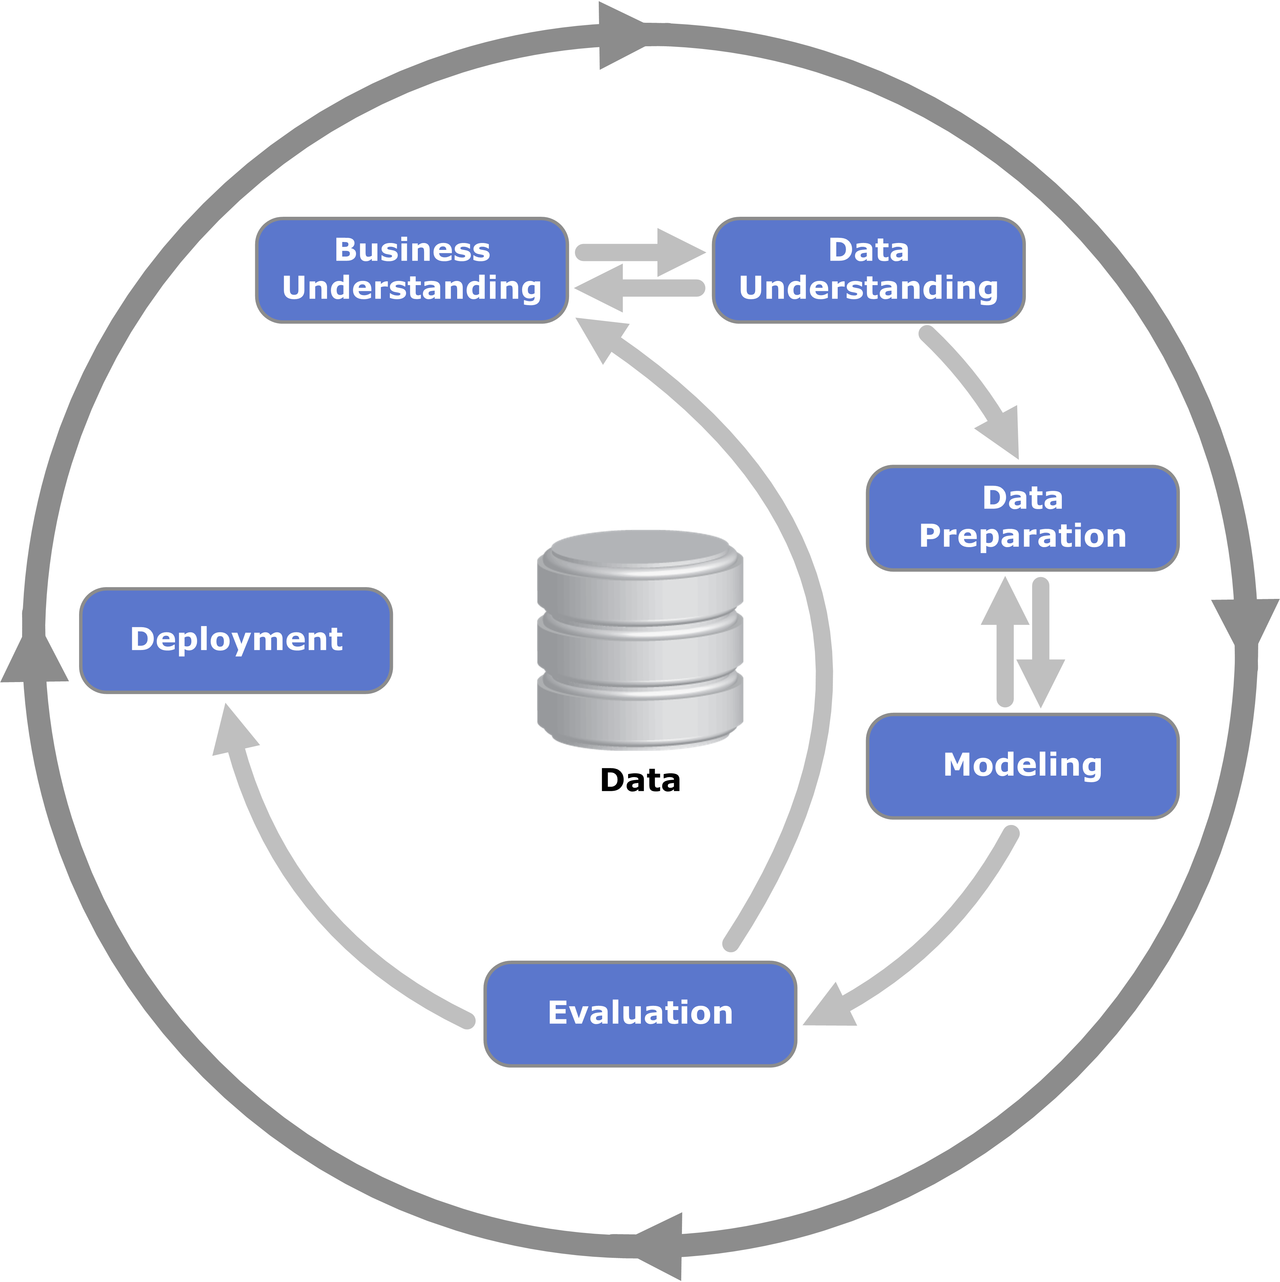
\includegraphics[width=0.5\linewidth]{images/crispdm.png}
    \label{fig:crispdm}
\end{figure}

\subsubsection{Business Understanding}
With the increase in usage of e-commerce, consumers can now interact with businesses, especially in online settings. This relies on a need for a platform that can be convenient for customers in online shopping transactions. In this digital landscape, product reviews can play a critical role in shaping consumer and business decision, offer valuable insights about the quality of resources, gain a better understanding of the experiences of specific users, and gauge the overall satisfaction levels of those buying and selling. Therefore, both customers and businesses can take advantage of the abundance of feedback to make well-informed decisions, make improvements in their products and services, and enhance customer engagement. 

\subsubsection{Data Understanding}
The dataset that is utilized is a collection of product reviews from the e-commerce platform Amazon. It exhibits a significant volume of data and comprises of various columns that provide insights into reviewer demographics, product details, ratings, and overall sentiments. The columns are as follows: reviewerID, asin, reviewerName, vote, style, reviewText, overall, summary, unixReviewTime, reviewTime, image. Notably, the column of ``verified user'' indicates whether or not the reviewer actually purchased the product through the platform, further adding credibility to their feedback. Based on the problem defined in the Business Understanding phase, we have determined that the most important features to keep are `Overall', `Verified', `ReviewText', and `Summary'.
`Overall' is the total rating the customer reviewed. `ReviewText' is the text of the review, and `Summary' is a short description of the review. 

\subsubsection{Data Preparation}
The steps to prepare the data requires several important steps. This ensures that the dataset is ready for data analysis. Firstly, the data needs to be cleaned and transformed which involves handling missing values, removing any duplicates, and downsampling the data to account for class imbalance. Next, sentiment values will be based on the review ratings, which are assigned as positive, neutral, or negative to each review. There will be sentence preprocessing techniques including the use of regular expression (regex) for character removal, NLTK for removing stop words, stemming, and lemmatization. These methods will be applied to streamline the textual data. More text processing techniques like bag-of-words or Term Frequency-Inverse Document Frequency (TF-IDF) may also be employed to convert the categorical data into a numerical format. Alternatively, splitting the data into training and testing sets can be defined for model evaluation. 

\subsubsection{Modeling}
Several classification algorithms will be considered and used for sentiment analysis. This includes logistic regression, Naive Bayes, Decision Trees, and Support Vector Machine (SVM). More complex models like Recurrent Neural Network (RNN) or Long Short-Term Memory (LSTM) could also be explored for sequence-based sentiment analysis if timing and resources are sufficient. Furthermore, ensemble techniques may be applied to enhance the predictive performance of each model.

\subsubsection{Evaluation}
The performance of the model will be evaluated using metrics such as accuracy, confusion matrix, precision, recall, and F1 score. These will be presented in a classification report. Alternatively, more evaluation metrics such as cross-validation, log loss, or Receiver Operating Characteristic Area Under the Curve (ROC AUC) could be utilized, which would work effectively for deep learning models. 

\subsubsection{Deployment}
After the model is developed, the contributions of the group members for this project will be expanded and highlighted based from the insights gained from the sentiment analysis and potential implication for businesses. The model performance will be monitored over time and will be tracked using metrics discussed earlier including accuracy, latency, and concept drift. We will also set up alert systems and establish them to notify stakeholders if performance from the model is performing below predefined thresholds and standards. If there is such a case, there will be contingency plans to address any issues and ensure the continued efficacy of the models created and deployed. 

\subsection{Project Organization Plan}
To organize our project we will break all the tasks down in a hierarchical pattern. This pattern is known as the Work Breakdown Structure. The tasks that need to be completed in order to fulfil the project development methodology above are detailed below:

\begin{enumerate}
    \item The first step in the process is the \textit{Business Understanding} phase, which involves comprehending the business objectives and requirements. Here, we will define the problem statement, identify any key stakeholders, and determine how data analytics and sentiment analysis can address business needs effectively. 
 
    \item The next step is \textit{Data Understanding}. In this step, we will use the data to gain insights about its structure, any interesting contents, and the overall quality of the data. We will create exploratory data analysis to understand the distributions of the data, identify any patterns, and uncover potential issues, challenges, and biases. 
    
    \item In the \textit{Data Preparation} stage, we will proceed with cleaning, transforming, and preprocessing the data as neccessary after we have understood and analyzed the data. This involves handling missing values, removing duplcates, standardizing formats, and encoding categorical variables. In addition, the data will be split into training and testing sets so that the model can be developed effectively and evaluated successfully as well. 
    
    \item Once the data is prepared, the \textit{Modeling} phase is when the team will determine the appropriate techniques and models are used, depending on the research topic and the data. Various and multiple algorithms such as classification, clustering, and ensemble, will be considered. Individually, each member will develop one or more models to address the business objectives.
    
    \item In the \textit{Evaluation} step, the models will be tested based on performance metrics like accuracy, precision, recall, and F1 score. This evaluation step will enable the comparison of different models and their respective level of performance. The model that exhibits the best performance will usually be selected for deployment. 
    
    \item The final step is the \textit{Deployment} phase. Here, the selected model will be deployed into a real-world application or into a production environment to begin with. Deployment integrates the model into existing systems that work and sets up monitoring algorithms to track and check performance metrics over time. This will establish protocols in the case the model needs maintenance or updates if needed. 
\end{enumerate}

By following these six steps of the CRISP-DM methodology, our project aims to follow each step to ensure the objectives and goals are met so that we can deliver insights through these data analytics solutions. The breakdown of our project can be seen in Figure \ref{fig:work-breakdown-structure}.
    
\begin{figure}[!htb]
    \centering
    \caption{Work Breakdown Structure for E-Commerce Sentiment Analysis}
    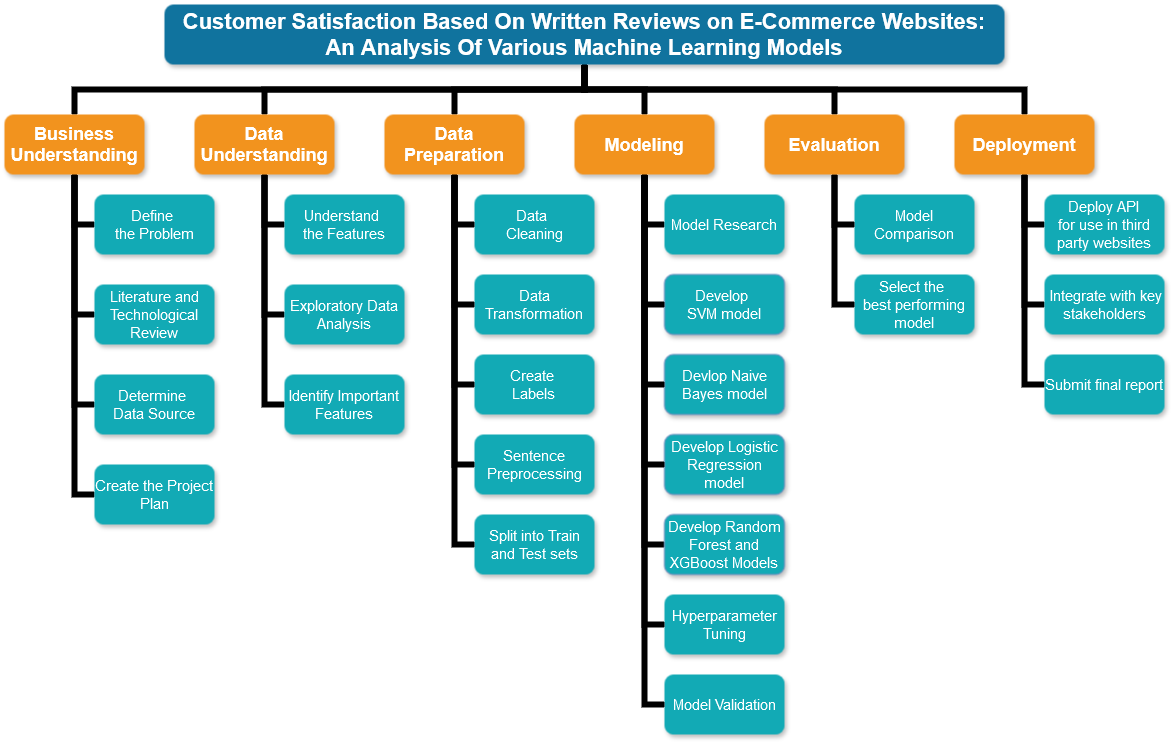
\includegraphics[width=1\linewidth]{images/WBS.png}
    \label{fig:work-breakdown-structure}
\end{figure}


\subsection{Project Resource Requirements Plan}
\subsubsection{Hardware}
To run the various machine learning models, we require some powerful hardware. The two main pieces of hardware are Google Colab for running code and Git-LFS for data storage. A summary of our hardware requirements is detailed in Table \ref{tab:hardware}.

For Google Colab, our specification is that it is a cloud-based Jupyter notebook environment with access to GPU and TPU resources. The cost is free based on the available resources, however we are aware that paid plans offer extended usage and additional features. Overall, Google Colab provides a convenient platform for developing and executing machine learning workflows. It is also integrated with Google Drive, which we will use our school student accounts to facilitate data storage and collaboration. This will allow access to GPU and TPU for model training. 

For Git-LFS, the specification is that it is a version control system extension for managing large files efficiently. It is free and open-source, and the justification for its usage is that it enables storage and management of large datasets and other files within the Git version control system and environment.

\begin{table}[!htb]
    \centering
    \caption{Hardware Requirements}
    \begin{tabular}{cccc}
    \hline
         Service& Configuration & Purpose & Cost \\ 
         \hline
         Local Machines & various & Coding platform & Owned (free)\\
         Google Colab & T4 GPU (16GB RAM) & Compute platform & Free \\
         Google Colab & A100 GPU (80GB RAM) & Compute platform & \$9.99/100 compute units \\
         Git-LFS & 1GB Storage & Data Storage & Free* \\ 
         \hline
    \end{tabular}
    \tablenote{*Paid version available, A100 GPU utilizes approximately 11 compute units/hour}
    \label{tab:hardware}
\end{table}

\subsubsection{Software}
To train and run the models, we need to utilise various software tools that provide the appropriate software development environment. The primary language used is Python, using the Anaconda python distribution. The anaconda python distribution provides us with many useful libraries such as Pandas, NumPy, SciKit Learn, and more. One of the key features of the Anaconda distribution is the inclusion of Jupyter Notebook, which is a powerful visual Python REPL tool. Besides Python, we also used GitHub for code collaboration, Google Docs, Discord for communication, and OverLeaf for collaborative report writing. A full list of software tools used can be found in Table \ref{tab:software}.


\begin{table}[!htb]
    \centering
    \caption{Software Requirements}
    \begin{tabular}{cccc}
    \hline
         Service& Configuration  &Purpose& Cost \\
         \hline
         Python & Version 3.11  &Coding platform& Free \\
         Pandas & Version 2.1.1  &Working with datasets& Free \\
         NumPy & Version 1.26.1  &Advanced mathematics& Free \\
         Scikit-Learn & Version 1.3.1  &Basic machine learning& Free \\
         CUML & Version 20.04.00  &GPU accelerated machine learning& Free \\
         NLTK & Version 3.8.1  &Language processing& Free \\
         Regex & Version 2023.10.3  &Text manipulation& Free \\
         Jupyter Notebook & Version 6.5.4  &Code REPL platform& Free\\
         Google Colab & N/A  &Code REPL platform& Free*\\
         Kaggle Notebook & N/A  &Code REPL platform& Free*\\
         GitHub & N/A  &Code collaboration& Free \\
         Overleaf & N/A  &Report writing collaboration& \$9/month \\ 
         \hline
    \end{tabular}
    \tablenote{*Paid version available}
    \label{tab:software}
\end{table}

There are no specific licenses that are required for the mentioned tools and platforms. Most of these tools are open-source and/or offer free access for individual and academic use. However, organizations or business may need to review the licensing agreements or the terms of service should they want to view the policies and data privacy regulations. 

Ultimately, the selected hardware, software, and tools provide an extensive understanding for the infrastructure used to develop and deploy machine learning models efficiently. These resources will ensure easy collaboration while minimizing costs and time. 

\subsection{Project Schedule}
Gantt charts help visualize the project schedule with tasks, timelines, responsible team members, and the status of the deliverables. This view of the tasks help see an overall picture of the project from the start to the planned end date of the project. Though this view is great at visualizing the overall timeline of the project, it does not immediately show the effect of a delay on a critical part of the project. The main con against Gantt charts is that they do not show the critical task dependencies of the project as a whole. To see this, we can use a PERT chart.

PERT (Program Evaluation Review Technique) charts allow the project organizers to lay out all the tasks on a dependency graph with each tasks start and end dates. Based on these dates, we can calculate the amount of slack a certain task has. Furthermore, the PERT chart allows us to identify the critical path. The critical path is the series of tasks, that if any one of them has a delay, it will delay the entire project. 

The Gantt/PERT charts for this project can be seen in Figures \ref{app:fig:gantt} and \ref{app:fig:pert}, respectively.


\section{Data Engineering}

\subsection{Data Process}
The process of collecting the raw datasets and preparing training, validation, and test datasets for data analytics involves several steps. The overview of the process can be summarized below: 

The raw dataset is collected from Amazon Product Reviews and includes various products, categories, and user-generated contents. The raw dataset undergoes preprocessing steps to clean and refine the data, where irrelevant columns are removed and sentence preprocessing techniques like punctuation removal, lowercase conversion, and tokenization applied to standardize the data. The preprocessed dataset is transformed into numerical representation that is suitable for analysis and modeling. The two common transformation techniques are Bag-of-Words (BoW) and Term Frequency-Inverse Document Frequency (TF-IDF) and applied to convert the text data into feature vectors. The transformed dataset is split into training, validation, test sets to facilitate model development, validation, and evaluation at 70 percent, 15 percent, 15 percent respectively. It's important to note that each model had its own interpretation and exhibited closely related values to the numbers in the respective training, validation, and testing phase. This will allow appropriate distribution of data across each subset. The training set will train the machine learning model, the validation set will fine-tune the hyperparameters and assess performance of the model, the test set will evaluate the final model's performance on unseen data. 

\subsection{Data Collection}

The raw dataset that is utilized in this research is the Amazon product review produced by \textcite{ni2019justifying_dataset}, which contains a large collection of reviews that cover many product categories, providing a thorough resource for data analysis. The quantity of this raw dataset ranges from thousands to millions of reviews and includes several parameters that highlight different aspects for each unique product review, see Table \ref{tab:amazon_review_cols}. The product categories selected for analysis can be found in Table \ref{tab:amazon-categories}.

For simplicity of the project, we combined all the reviews from all categories into a single file. This file was created by extracting the reviews from the GZIP-compressed JSON file using python and concatenating them into a single Pandas DataFrame. This DataFrame was saved to disk as `combined.csv' and pushed to our GitHub repository. The combined data has a total of  12 columns (See Table \ref{tab:amazon_review_cols}) and 749,404 rows (See Table \ref{tab:amazon-categories}). An excerpt of the original dataset can be seen in Figure \ref{fig:original-dataset}

\begin{table}[!htb]
    \centering

    \caption{Common fields in all reviews}
    \begin{tabular}{ccc}
        \hline
        Column name & DataType  &Description\\ 
        \hline
        overall & Float  &Score from 0 to 5\\
        verified & Boolean  &True or false, see \cite{amazon2024help_verified}\\
        reviewTime & date  & The date when the review was made\\
        reviewerID & string  & Unique identifying string for user\\
        asin & string  & Unique identifying string for product\\
        reviewerName & string  &The name of the user leaving the review\\
        reviewText & string  &The main text of the review\\
        summary & string  &The summary or title of the review (optional)\\
        unixReviewTime & timestamp  &unix time stamp\\ 
        vote & int & Number of people who found the review helpful \\
        style & Dictionary & Selection type\\
        image & link & The link of an image that a user used in their review\\
        \hline
    \end{tabular}
    \label{tab:amazon_review_cols}

\end{table}

\begin{table}[!htb]
    \centering

    \caption{Selected categories for analysis}
    \begin{tabular}{cc}
        \hline
        Category name & Number of reviews  \\ 
        \hline
        Amazon Fashion & 3,176  \\
        All Beauty & 5,269  \\
        Appliances & 2,277  \\
        Arts, Crafts, and Sewing & 494,485  \\
        Musical Instruments & 231,392  \\
        Software & 12,805  \\
        Total & 749,404 \\
        \hline
    \end{tabular}
    \label{tab:amazon-categories}

\end{table}

\begin{figure}[!htb]
    \centering
    \caption{Original Dataset first 5 rows}
    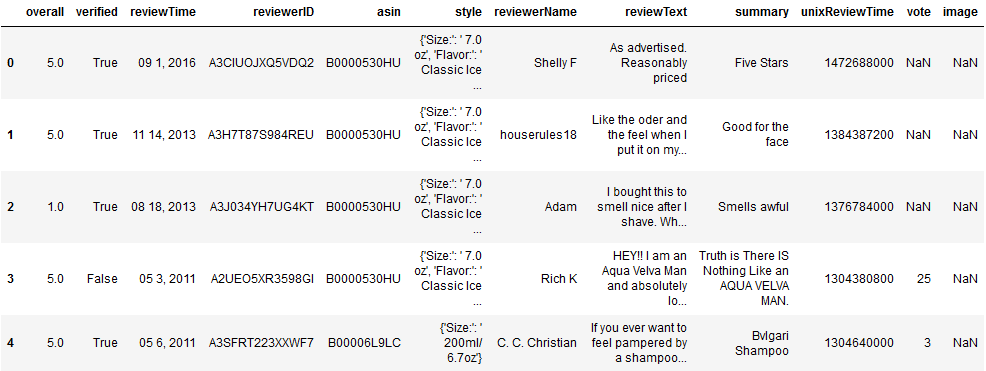
\includegraphics[width=0.9\linewidth]{images/original-dataset.png}
    \label{fig:original-dataset}
\end{figure}

\subsection{Data Preprocessing}
After collecting the raw datasets, the next step is to preprocess which includes cleaning and validating the data. This ensures that the quality is standardized and easier to interpret. The preprocessing steps include:

Merging from multiple categories means we will combine the data from multiple product categories to create a dataset that is comprehensive and includes all features for analysis. To fix null values we identified and addressed null and missing values in the data so there is consistency. This included around 400 empty reviews/summaries. Checking for the duplicates in the original dataset, we found there were 58,255 duplicate entries, see Figure \ref{fig:duplicates}. These duplicates were dropped, leaving the DataFrame with 691,149 rows. In addition, we removed irrelevant columns for the features that did not contribute to the analysis. This included every column outside of overall, verified, reviewText, and summary. After these basic preprocessing steps, we ended up with Figure \ref{fig:subset-columns}.

\begin{figure}[!htb]
    \centering
    \caption{Duplicates in the dataset}
    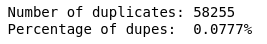
\includegraphics[width=0.4\linewidth]{images/duplicates.png}
    \label{fig:duplicates}
\end{figure}

\begin{figure}[!htb]
    \centering
    \caption{Dataset after removing unnecessary columns}
    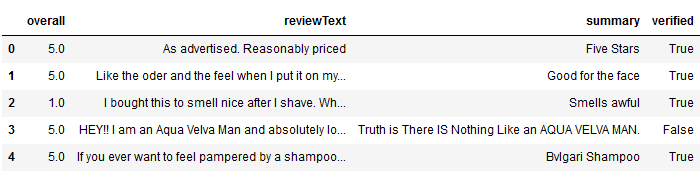
\includegraphics[width=0.9\linewidth]{images/subset-columns.png}
    \label{fig:subset-columns}
\end{figure}


For the purposes of testing the code, we used stratified subsamples of the dataset. This allowed us to test our code quickly and iteratively before running on the full dataset while still preserving the overall important characteristics of the dataset.

\subsection{Data Transformation}
The step that follows preprocessing is transforming the data. This is where the clean and validated data will undergo transformation into desired formats for appropriate use, enabling the data to be structured and represented for analysis and modeling. 

The sentiments are applied to the dataset based on Formula \ref{eq:sentiment}.

\begin{equation}
\text{sentiment} = \begin{cases}
-1 & \text{overall} < 3\\
0 & \text{overall} = 3 \\
1 & \text{otherwise}
\end{cases} 
\label{eq:sentiment}
\end{equation}

An overall score of 1 and 2 are negative sentiments, a score of 3 is labelled as neutral sentiment, and scores 4 and 5 are positive sentiments. Additionally, the `reviewText' and `summary' columns were combined to allow us to perform more thorough analysis. An example of how the dataframe looks can be seen in Figure \ref{fig:transform-cols}.

\begin{figure}[!htb]
    \centering
    \caption{Dataset after transforming the columns}
    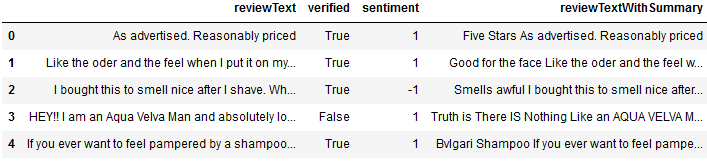
\includegraphics[width=0.9\linewidth]{images/transformed-columns.png}
    \label{fig:transform-cols}
\end{figure}

Text preprocessing techniques such as regular expressions (regex) and Natural Language Toolkit (NLTK) stopwords removal were applied to clean the data of its text. In addition, other methods to clean the text even more include stemming or lemmatization to standardize the text and reduce dimensionality. By executing these steps the raw dataset is transformed into a more clean dataset that is ready for analysis. A comparison of these preprocessing type can be seen in Figure \ref{fig:preprocessed-data}.

The datasets are transformed into a Bag-of-Words (BoW) representation using `CountVectorizer', which is a tool that converts text documents into numerical feature vectors. In doing so, the presentation captures the frequency of words within each review and allows for the creation of a sparse matrix of features that can be used for analysis. 

In addition to BoW representation, the dataset can be transformed using TF-IDF (Term Frequency-Inverse Document Frequency) vectorization. This type of method values the importance of words within the entire text, with more common words being weighed down and rare words being highlighted and carrying more significance. Since both the TF-IDF and BoW vectorizers use the same underlying principle, i.e. word frequency, the size of both vectorizations on a certain text will be the same.

For example, one of our conversions used the stemming technique followed by vectorization using the TF-IDF vectorizer. Doing so transformed it into a sparse matrix of 150,189 numerical features, making it possible for the selected algorithms to actually train on the data. See Figure \ref{fig:vectorspace} for the size of all vector spaces. Due to an oversight that went uncaught, the punctuation removal code was faulty, resulting in a larger feature space than the unprocessed text. This was due to the false assumption that a majority of the text available would follow proper grammatical rules. We realized the fault too late into the project. Currently, the punctuation removal replaces the character with `'. By doing so, it creates extra words in the feature space by combining words separated by characters such as commas without a space. In the future, this can be fixed by replacing punctuation marks with a `space' character rather than outright removing it.

\begin{figure}
    \centering
    \caption{Feature space of all columns transformed}
    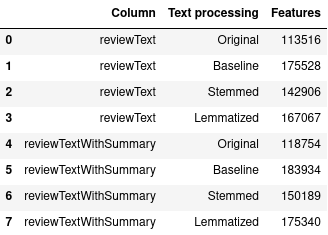
\includegraphics[width=0.5\linewidth]{images/vector_spaces.png}
    \figurenote{Due to coding oversight, punctuation removal actually increases the feature space}
    \label{fig:vectorspace}
\end{figure}

\subsection{Data Preparation}

The transformed dataset is split into three subsections: training, validation, and testing sets. The exact size of each subset is defined prior to ensure appropriate distribution of data for model training, validation, and evaluation. The proposed split ratios are 70\% for the training and 15\% each for the testing and validation sets, see Table \ref{tab:splitratio}.

\begin{table}[!htb]
    \centering
    \caption{Split ratios on dataset}

    \begin{tabular}{ccc}
    \hline
    Set & Percentage & \# of Rows\\
    \hline
    Training & 70 & 483,438 \\
    Testing & 15 & 103,594 \\
    Validation & 15 & 103,594 \\ \hline
    \end{tabular}

    \label{tab:splitratio}
\end{table}

The transformed dataset split into the training, validation, and testing sets is made into the defined split sizes. This split ensures each subset contains representative samples of the data and facilitates accurate modeling and evaluation. By preparing training, validation, and testing sets from the transformed dataset, the research aims to provide availability of properly partitioned data for development and evaluation, contributing to reliability of findings. 

The goal of using a three way split is to be able to perform valid comparisons between the base model and hyperparameter tuned models. To do so, first a baseline model is trained on the train set and evaluated on the validation set. This is a basic model that used its default parameters. Next we perform either a grid search cross validation or a random search cross validation based on the parameter grid size and the complexity of the model. This grid search is fitted on to the validation set. Finally, we use the best parameters from the grid search on a new instance of the model. This new model is trained on the train set and finally evaluated on the test set.

Though in this paper, it is implied that TF-IDF/BoW vectorization was applied before data splitting, in reality this caused multiple out of memory errors at time of data splitting. So, instead we performed the splitting first and applied the vectorizations afterwards to each split.

\subsection{Data Statistics}
To gain a better understanding of the data, we performed some statistical analysis. Since we are performing analysis on textual data, the main statistics we check are review lengths and word frequency/word cloud. First, we can just get a basic understanding of the data by taking a look at the length of the reviews, see Figure \ref{fig:box-plot}.  The outliers from the above graph were removed as it made the graph hard to read. The longest of these reviews was 5,118 words long. To understand the effect of these outliers on our dataset, we explored what these `long reviews' were.


\begin{figure}[!htb]
    \centering
    \caption{Box plot of review lengths}
    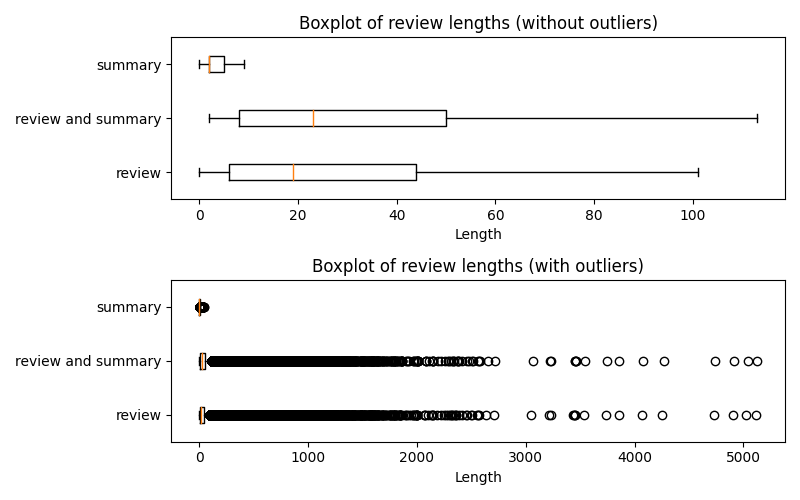
\includegraphics[width=0.8\linewidth]{images/results/review_length_boxplot.png}
    \label{fig:box-plot}
\end{figure}

Based on this finding, we did an analysis of the lengthy reviews. There are 16 reviews that are longer than 3,000 words. Reviews longer than 500 words number nearly 3,420 (around 0.495\% of the dataset). An excerpt from the longest review and a wordcloud of all reviews longer than 500 words can be seen in Figure \ref{fig:long-reviews}.

\begin{figure}[!htb]
    \centering
    \caption{An excerpt from a very long review and a wordcloud of all reviews longer than 500 words}
    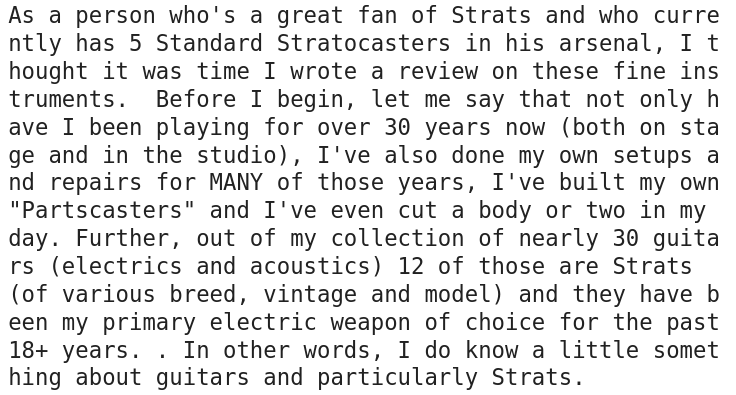
\includegraphics[width=0.39\linewidth]{images/large_review_sampe.png}
    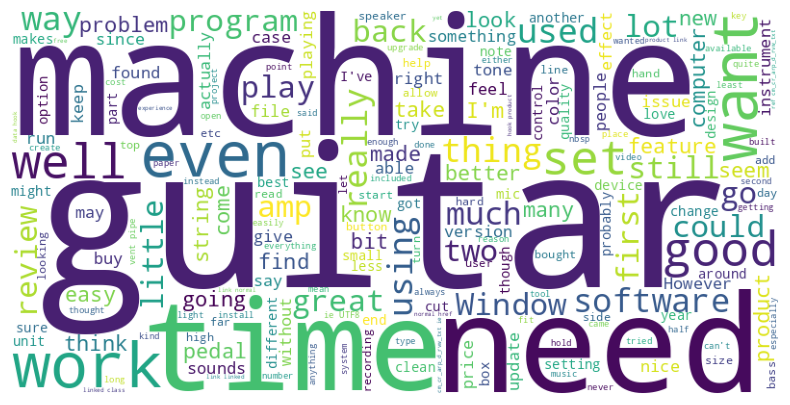
\includegraphics[width=0.39\linewidth]{images/long_reviews_word_cloud.png}
    \label{fig:long-reviews}
\end{figure}

Further analysis of these longer reviews displayed to us that they would not pose a challenge in our modelling as the data in the lengthy reviews themselves was valuable. Moreover, the grammar of the long reviews matched regular English speech, i.e. The inclusion of these reviews would not significantly impact the dictionaries used by the Bag of Words `CountVectorizer' or the TF-IDF `TFIDFVectorizer'.

\begin{figure}[!htb]
    \centering
    \caption{Distribution of product review ratings and sentiments of selected categories}
    
\includegraphics[width=0.9\textwidth]{images/selected_categories_ratings_distribution.png}
    \label{fig:selected-categories-dist}
\end{figure}

Recalling Figure \ref{fig:j_shaped_distribution}, which was calculated over the entire super set of the available data, we also wanted to figure out the distribution in our selected categories. This can bee seen in Figure \ref{fig:selected-categories-dist}. Comparing the 2 figures, we can see that the the `J shape' of our distribution becomes more extreme. 

Word clouds for the raw text grouped by class were created and are shown in Figure \ref{fig:wordcloud-baseline}. It can be seen that while positive reviews have a large variety of words, negative and neutral reviews have a very similar set of words. In an attempt to remedy this, we decided to combine the reviewText column with the summary column. The resulting word cloud can be seen in Figure \ref{fig:wordcloud-summary}. This can also be seen in the bar plot in Figure \ref{fig:top-10-barplot}.

\section{Model Development}
\subsection{Model Proposals}
The goal of this project is to create a model based on supervised learning techniques in order to accurately predict the sentiment of users based on their reviews. To obtain the best results, we plan on using supervised learning, where the labels are the sentiments and the features are the reviews. The Amazon Product Review dataset has a large variety of categories and a wide range of reviews, making it suitable to use in this regard. The models proposed for our project range from simple models like Logistic Regression to complex models like XGBoost. The selected models are described in the following sections in regards to their mathematics and how they are applicable to the problem we are trying to solve. 

\subsubsection{Logistic Regression}
Logistic Regression is a popular classification algorithm due to its simplistic nature \parencite{scikit-learn}. Some of the advantages of Logistic Regression is that it is efficient, easy to interpret, and works well with linear datasets. However, it does not work well in high dimensions, requires large sample size, and often fails to capture complex relationships. Nonetheless, it is a good model for classification problems. Mathematically, logistic regression estimates a linear function \parencite{prabhat2017sentiment}. While it is generally used for binary classification, it can be used for the multiclass case as well, which is used in this project. In the case for multinomial logistic regression, the softmax (Equation \ref{eq:lr-softmax}) function is used to map the input features to a probability value between 0 and 1, where x represents the dot product between the weights and features.






\begin{equation}
    s(x_i)=\frac{e^{x_i}}{\sum_{j=1}^{n}e^{x_j}}
    \label{eq:lr-softmax}
\end{equation}

The cost function, shown in Equation \ref{eq:lr-logloss}, details the negative log likelihood function. By taking the partial derivative with respect to the weights, the gradient is able to be calculated. Using this, gradient descent is able to be performed, which will update the weights for the model until convergence (or maximum iterations).








\begin{equation}
J(\theta) = -\left[
\sum\limits_{i=1}^{m} \sum\limits_{k=1}^{K}
1 \left\{ y^{(i)} = k \right\} 
\log \frac{\exp\left(\theta^{(k)\top}x^{(i)}\right)}
{\sum_{j=1}^{K}\exp\left(\theta^{(k)\top}x^{(i)}\right)}
\right]
\label{eq:lr-logloss}
\end{equation}

Once the optimal weights are found from the gradient descent algorithm, the model uses a combination of thresholds and the One vs Rest implementation to make predictions. The threshold, generally set to 0.5, is used to determine the class based on their probability. Figure \ref{fig:logreg_process} details the general process taken for the logistic regression algorithm.

\begin{figure}[!htb]
    \centering
    \caption{Logistic Regression Algorithm Process}
    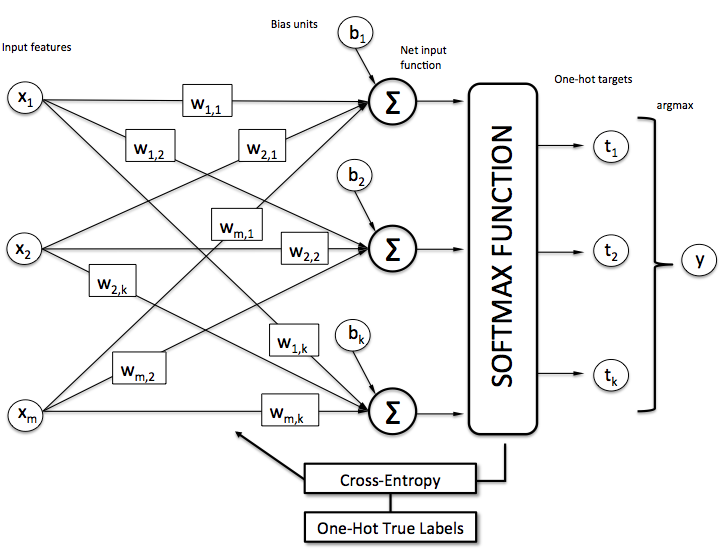
\includegraphics[width=0.5\linewidth]{images/logreg_process.png}
    \label{fig:logreg_process}
\end{figure}

The One vs Rest implementation is a commonly used method that creates a model for each class and outputs a prediction based on the highest probability amongst all models \parencite{Kumar_2023}. In the case for this project, a One vs Rest implementation will create models for the following classes: Positive vs Not Positive, Neutral vs Not Neutral, and Negative vs Not Negative. Then, the class with the highest probability amongst all models is selected. The visual representation for the general One vs Rest implementation can be seen in Figure \ref{fig:ovr}.
\begin{figure}[!htb]
    \centering
    \caption{One vs Rest}
    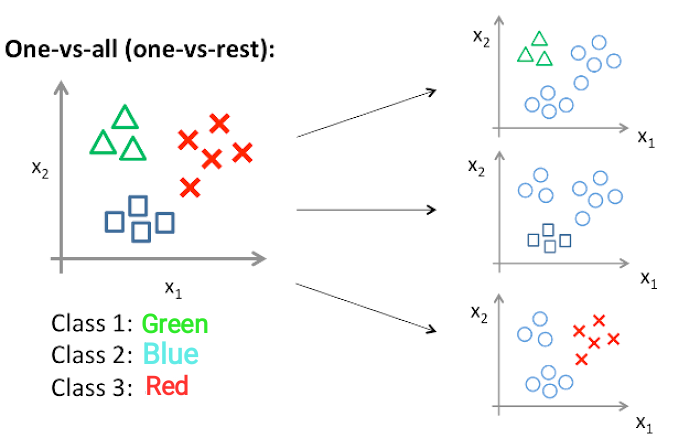
\includegraphics[width=0.5\linewidth]{images/ovr.png}
    \label{fig:ovr}
\end{figure}

\subsubsection{Support Vector Machines}

Support Vector Machines (SVM) are a supervised learning model that can be used for classification. The model works by finding the optimal hyperplane that separates the data into one of two classes. The goal is to find a hyperplane that maximizes the margin between the two classes. The margin lines coincide with a particular data point, these data points are known as the support vector \parencite{cortes1995support}. Take a look at Figure \ref{fig:svm} for a visual representation of this.

\begin{figure}[!htb]
  \centering
  \caption{A visual representation of a SVM}
  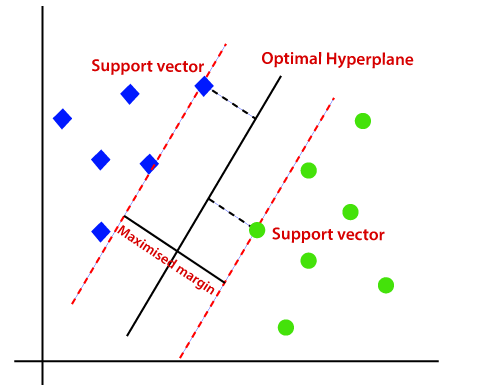
\includegraphics[width=0.4\textwidth]{images/svm/svm.png}
  \label{fig:svm}
\end{figure}

According to \textcite{scikit-learn}, the primal formulation of support vector classifiers is given by Equation \ref{eq:svm-primal}. This equation states that $||w||^2$ must be minimized, with some slack $\zeta_i$. The slack or `penalty' amount is controlled by the $C$ parameter. The rule that the minimization is subject to try to maximize the margins. By balancing this minimization and maximization, we are able to solve the problem.

\begin{align}
\begin{aligned}
& \min_ {w, b, \zeta} \frac{1}{2} w^T w + C \sum_{i=1}^{n} \zeta_i\\
\begin{split}
\textrm {subject to } & y_i (w^T \phi (x_i) + b) \geq 1 - \zeta_i,\\
                      & \zeta_i \geq 0, i=1, ..., n
\end{split}
\end{aligned}
\label{eq:svm-primal}
\end{align}

This problem can be further broken down in it dual form, given by Equation \ref{eq:svm-dual}.

\begin{align}
\begin{aligned}
& \min_{\alpha} \frac{1}{2} \alpha^T Q \alpha - e^T \alpha\\
\begin{split}
\textrm {subject to } & y^T \alpha = 0\\
                      & 0 \leq \alpha_i \leq C, i=1, ..., n
\end{split}
\end{aligned}
\label{eq:svm-dual}
\end{align}

Where $e$ is a ones vector, $Q$ is a square matrix of size $n$ such that each element of $Q$ is given by Equation \ref{eq:svm-qarray}. The $\alpha$ terms are bounded by $C$. The dual representation in Equation \ref{eq:svm-dual} works on the principle that the training vector can be mapped into an infinite dimension space by the kernel function $\phi$.

\begin{equation}
Q_{ij} \equiv y_i y_j K(x_i, x_j) 
\label{eq:svm-qarray}
\end{equation}

After solving the dual problem, we can make the decision using the decision function given by Equation \ref{eq:svm-decision}. This works by check the sign of the answer, positive is one class while negative is the other class.

\begin{equation}
\sum_{i\in SV} y_i \alpha_i K(x_i, x) + b
\label{eq:svm-decision}
\end{equation}

In terms of the problem we are solving, i.e. multiclass sentiment analysis of textual data, SVM is a very good model as vectorizing the text data using either `TF-IDF' or `Bag of Words' transforms that data into a very large vector space, which SVM handles very well. In extended literature, this model is also justified for use in sentiment analysis, such as in the paper by \textcite{gupta2017study}, where the SVC classifier achieved an average accuracy of 85\% on classifying the sentiment of tweets. For preliminary testing we used the SVC function provided by the SciKit-Learn library, where as in the baseline and final models, we used the SVC function provided by `cuML'. In the case of `cuML', the default multiclass decision strategy is `One versus Rest' strategy, see Figure \ref{fig:ovr}.


\subsubsection{XGBoost}
XGBoost is a popular supervised tree based model that is frequently utilized for classification. It is known for being very fast, maintain high accuracy, handle large datasets, and prevents under fitting \parencite{GuptaComparisons}. It is both compute and memory intensive. This model particularly works well with imbalanced datasets. Since we are dealing with a large and imbalanced dataset of Amazon reviews, this model can be considered ideal for this situation. Since this is a case of multi-class classification, we apply the multi:softmax function. The function just returns class which contains the highest probability \parencite{forecastegy_xgboost_multiclass_classification}. This takes the probabilities of every possible outcome associated with a specific review from the dataset, and assigns it the sentiment with the largest probability. 

In multi-class classification, softmax and cross-entropy are put together for use since this model is tree based. The softmax function is responsible for providing the probability distribution provided across all the sentiment outputs from the model. Cross entropy checks to see how well the probability distribution performs given the true label \parencite{charanhu_2023}. 

\textcite{dahal2017softmax} provides the theoretical understanding of how cross entropy and softmax can be combined. The equation  of softmax is as follows:
\[
p_i = \frac{e^{a_i}}{\sum_{k=1}^N e^{a_k}}
\]
The derivative of this function for both i = j, and i does not equal j is represented as below:
\begin{equation}
\begin{cases}
p_i(1-p_j) & \text{if } i = j\\
-p_j \cdot p_i & \text{if } i \ne j
\end{cases}
\label{eq:xgboost_cases}
\end{equation}
The cross entropy equation is represented as follows:
\begin{equation}
\sum_{r} \delta_{rk} P_k
\end{equation}
The derivative of the cross entropy results in:
\begin{equation}
-\sum y_{k}\frac{1}{p_{k}} \times \frac{\delta p_{k}}{\delta o_{i}}
\label{eq:dercrossent}
\end{equation}







Combining Equation \ref{eq:dercrossent} with Equation \ref{eq:xgboost_cases}, the combined results are as follows:

\begin{align}
   & -y_i(1-p_i)-\sum\limits_{k \ne i} y_k \frac{1}{p_k}(-p_k \cdot p_i)\\
   & = p_i\left(y_i + \sum\limits_{k \ne 1} y_k\right) - y_i
\end{align}

















XGBoost is an ensemble technique of Decision Trees. It represents the boosting ensemble algorithm. In this model, decision trees are built behind the scenes in a somewhat sequential manner. First one model gets trained behind the scenes and assigns weights depending on whether a learner is a strong or weak learner. The weak learner are typically given a higher priority. The next model is then responsible for learning from the previous one's mistakes and working to turn those weak learners into strong learners \parencite{wohlwend2023}. Effectively putting these weak learners together leads to a strong learner.

Various learners will categorized as either strong or weak learners pending pending on how well that specific tree assigns a sentiment to the reviews. The next tree will give more focus to the weak learners, and ensure that any misclassified reviews from the previous tree is corrected. 

\subsubsection{Naive Bayes}
Naive Bayes (NB) is a frequently employed supervised machine learning technique in sentiment classification because of its simplicity, efficiency, and capability to predict quickly. It operates on the principles of the Bayes Theorem, and it leverages conditional probability while also assuming all features are independent. Each feature is of equal importance and this ensures that no feature has more independence over others. By computing the posterior probability of a sample that part of a sentiment category based on the prior probability distribution, the Naive Bayes classifier calculates the sentiment category with the highest probability. This ultimately predicts the sentiment category for the given sample given the dataset.

The Bayes Theorem states that given $y$ (a class variable) and $x$ (a dependent feature vector for $x_1, x_2, x_3 \cdots x_n$), the formula can be seen in Equation \ref{eq:nb1} \parencite{scikit-learn}.

\begin{equation}
    P(y|x_1,\cdots , x_n) = \frac{P(y)P(x_1,\cdots , x_n|y)}{P(x_1,\cdots , x_n)}
    \label{eq:nb1}
\end{equation}

Along with the naive conditional independence assumption, it gives Equation \ref{eq:nb2} \parencite{scikit-learn}.

\begin{equation}
    P(x_i|y,x_1,\cdots , x_{i-1},x_{i+1},\cdots , x_n) = P(x_i|y)
    \label{eq:nb2}
\end{equation}


This can be simplified to Equation \ref{eq:nb3}
\begin{equation}
    P(y|x_1, \cdots , x_n) = \frac{P(y)\prod\limits_{i=1}^{n}P(x_i|y)}{P(x_1,\cdots , x_n)}
    \label{eq:nb3}
\end{equation}

Since the probability of $(x_1, x_2, \cdots x_n)$ is constant, this classification rule can be determined. As such this is the estimation to calculate $P(y)$ and $P(x_i | y)$ where $P(y)$ is the frequency of class y that is from the training set \parencite{scikit-learn}: 







\begin{equation}
    P(y|x_1,\cdots , x_n) \propto P(y)\prod\limits_{i=1}^{n}P(x_i|y)
\end{equation}

Which implies

\begin{equation}
    \hat y = \argmax_y P(y) \prod\limits_{i=1}^{n}P(x_i|y)
\end{equation}

There are several variants of the Naive Bayes algorithm. The different NB classifiers differ by the assumptions about the distribution in $P(x_i | y)$. Naive Bayes is particularly effective because it requires training data that is not too large, and works fast for its models. The Naive Bayes classifier, described by \textcite{li2020sentiment} operates by holding several assumptions. First, all samples are independent and identically distributed and the seconds is that it assumes features are independent of each other. 

There are various types of Naive Bayes algorithms tailored to different data distributions. Gaussian Naive Bayes is suitable for classification tasks with features assumed to follow a Gaussian distribution. Multinomial Naive Bayes is used for features that are discrete, most commonly for classification. Complement Naive Bayes is adapted from Multinomial Naive Bayes and is effective for datasets that are imbalanced. It utilizes statistics from complement of each class to determine the model weights. Bernoulli Naive Bayes is ideal for binary data and for multivariate Bernoulli distributions where features are binary. Finally, Categorical Naive Bayes is designed for data that is distributed categorically and each feature assumes its own categorical distribution \parencite{scikit-learn}. For the purposes of experimentation, only Gaussian, Multinomial, Bernoulli, and Complement are utilized.


\subsection{Model supports}
\subsubsection{Platform and Tools}
This project involves using machine learning in order to classify reviews as positive, neutral, or negative. The size of the data is large, so the datasets are stored as a CSV file on Google Drive and Github. For the coding of the models, a standard Jupyter Notebook (local, Google Colab, or Kaggle) was used. The list of hardware and software used in this project can be seen in Tables \ref{tab:hardware} and \ref{tab:software}.

Python is used as the primary coding language, as it has access to a wide variety of machine learning related libraries. Additionally, there are modules for storage and manipulation of data, matrix operations, and visualization, such as Pandas, NumPy, and matplotlib. The full list libraries used are shown in Table \ref{tab:libraries}.


\begin{table}[!htb]
    \centering

    \caption{Libraries and Modules}
    \scalebox{0.85}{
    \begin{tabular}{>{\centering\arraybackslash}p{0.15\linewidth}>{\centering\arraybackslash}p{0.2\linewidth}>{\centering\arraybackslash}p{0.3\linewidth}>{\centering\arraybackslash}p{0.3\linewidth}}

        \hline
        \multicolumn{2}{c}{Library} & Function/Class  & Usage\\  \hline
        \multirow{8}{*}{scikit-learn} & model\_selection & train\_test\_split & Splitting the data into train, validation, and test sets \\ \cline{2-4}
        & model\_selection & RandomizedSearchCV, GridSearchCV & Hyperparameter Tuning  \\\cline{2-4}
        & metrics & classification\_report, confusion\_matrix, accuracy\_score, roc\_auc\_score & Evaluation Metrics  \\ \cline{2-4}
        & feature\_extraction.text & CountVectorizer, TfidfVectorizer & Vectorize sentences  \\\cline{2-4}
        & linear\_model & LogisticRegression & Modeling  \\\cline{2-4}
        & svm & SVC & Modeling  \\\cline{2-4}
        & naive\_bayes & MultinomialNB, GaussianNB, BernoulliNB, ComplementNB & Modeling \\ \cline{2-4}
        & preprocessing & label\_binarize & Label encoding for ROC AUC Curve \\ \hline
        cuML & svm & SVC & GPU accelerated modelling \\ \hline
        XGBoost & xgboost & XGBClassifier & Modeling \\ \hline
        \multirow{2}{*}{NLTK} & corpus & stopwords & Sentence Preprocessing \\\cline{2-4}
        & stem & PorterStemmer, WordNetLemmatizer & Sentence Preprocessing \\ \hline
        Pandas & DataFrame & read\_csv, describe, dropna, head, etc. & Reading CSV data into dataframe. Manipulating the dataframe \\ \hline
        Regex & re & sub & Sentence Preprocessing \\ \hline
        matplotlib & pyplot.plt & plot, line, subplots, etc. & Visualizations \\ \hline
        Seaborn &  & heatmap & Visualizations \\ \hline
        wordcloud & wordcloud & WordCloud & Exploratory Data Analysis \\
        \hline
        pickle &  & dump, load & Model Persistence \\ \hline
    \end{tabular}
    }
    \label{tab:libraries}

\end{table}


\subsubsection{System Architecture}
After sentence preprocessing and vector transformation using CountVectorizer() and TfidfVectorizer(), the datasets were split into train, validation, and test sets using a ratio of 70:15:15. Then, Logistic Regression, Naive Bayes, SVM, and XGBoost were used to train the individual models.
Hyperparameter tuning was also performed for all of the models. GridSearchCV() and RandomizedSearchCV() were used to test multiple parameter combinations and cross validated them to find the optimal parameters. RandomizedSearchCV() is less exhaustive than GridSearchCV(), since it randomly selects n\_iter combinations instead of doing an exhaustive search. However, as a result, the parameters it finds may not be the most optimal. After finding the optimal parameters, the models are retrained and evaluated. Figure \ref{fig:model-arch} below details the general flow chart used for model training and evaluation.

\begin{figure}[!htb]
    \centering
    \caption{Modelling architecture}
    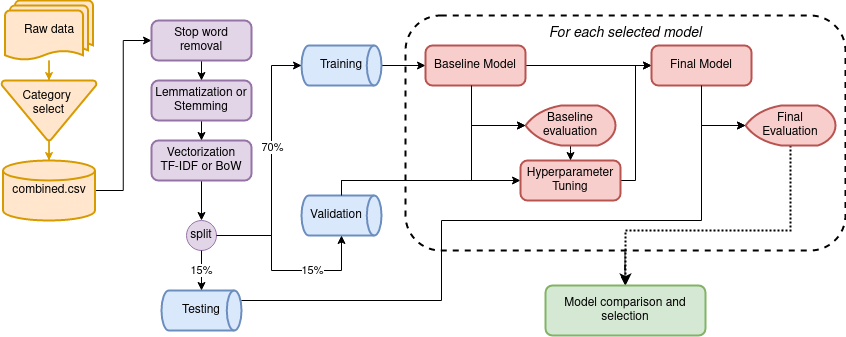
\includegraphics[width=\linewidth]{images/model_architecture.drawio.png}
    \label{fig:model-arch}
\end{figure}





\subsection{Model Comparison and Justification}

\subsubsection{Model Comparisons}
Machine learning models are important in predictions across various datasets. In this research, the models that were utilized were Logistic Regression, Support Vector Machine, XGBoost, and Naive Bayes. Each model was evaluated based on important criteria and evaluated to determine efficiency, effectiveness, and overall suitability for classification tasks. Model comparisons are done in Table \ref{tab:compare}.

\begin{table}[!htb]
    \centering

    \caption{Theoretical model comparison}
    \scalebox{0.8}{
    \begin{tabular}{ccccc}
        \hline
        Feature & Logistic Regression & SVM & XGBoost & Naive Bayes \\
        \hline
        Works well in high dimensions  & No & Yes & No & Yes\\
        Works well with categorical data & Depends on encoding & No & Yes & Yes \\
        Requires feature scaling & Yes & Yes & No & No \\
        Interpretability & High & Low & Low & High \\
        Handles imbalanced datasets & No & Yes & Yes & No \\
        Sample Size & Large & Small & Medium & Small \\
        Works with non-linear & No & Depends on kernel & Yes & Yes \\
        Training Time & Mid & Mid & High & Low \\ 
        Trainable parameters & Mid & Low & High & Low \\ 
        \hline
    \end{tabular}
    }

    \label{tab:compare}
\end{table}

\subsubsection{Model Justifications}
Logistic regression is a commonly used linear classification algorithm that is known for being simple and easy to interpret. But, its ability to work in high dimensional data settings is limited and struggles with non-linear relationships. On the other hand, Support Vector Machine (SVM) is a strong performer in high-dimensional data settings and is effective in handling non-linear data. This is primarily done through kernel functions. Although SVM is efficient in computing and is also robust to overfitting, SVM's interpretability is quite low, which is a potential challenge in making decisions. 

XGBoost is an ensemble learning technique, specifically a gradient boosting algorithmn that works well in handling categorical features and imbalanced data. As a result, this is a popular choice for prediction and known for its ability to capture interactions in the data. The drawback of using XGBoost is that is complex computationally and the time it takes to train data is high. This can be a problem for larger datasets. The other model is Naive Bayes, which is a probabilistic classifier. It is easy to implement and simple. Naive Bayes performs well for categorical data and has high interpretability, though its assumption states that feature must be independent, which limits its performance in predicting complex relationships.

\subsection{Model Evaluation Methods}

Class evaluation metrics are required to gain valuable insights into our model's classification performance. These metrics encompass various aspects of classification accuracy. They are True Positives, True Negatives, False Positives, and False Negatives. True Positives (TP) represent correct positive predictions made by the model, while False Positives (FP) indicate incorrect positive predictions. Similarly, True Negatives (TN) denote correct negative predictions, and False Negatives (FN) signify incorrect negative predictions.

In the case for our multiclass problem, we can substitute positives and negatives to `this class' vs `not this class'. In other words, the FP of a neutral sentiment would be reviews that are actually negative or positive being labeled as neutral.

These basic metrics form the basis of calculating model accuracy, precision, recall, and F1 score. Meanwhile the rate of false positives and true positives let us calculate the ROC curve. These metrics are discussed in detail below.

\subsubsection{Accuracy}
Accuracy is a common evaluation metric that measures the proportion of predictions accurately predicted. It is given by the following equation:
\[(TP + TN) / (TP + TN + FP + FN)\]

One thing to note is that accuracy does not work as well with imbalanced data, such as the dataset being used for this project, the Amazon Product Review data. Refer to the J-shaped distribution in Figure \ref{fig:j_shaped_distribution}. For our models, if we predict Positive sentiments accurately, but fail to predict neutral and negative sentiments, the overall accuracy will still be high, simply due to the large amount of Positive entries. As a result, the accuracy may be high but it becomes very clear that there is an issue with the models. This issue is somewhat remedied through the analysis of other evaluation metrics such as precision, recall, and F1 score.


\subsubsection{Precision, Recall, and F1 Score}

Precision is used to measure how often the model is correct when predicting the target. It does so by taking the proportion of True Positives vs all values predicted as positive. A low precision score implies that the model is predicting many False Positives. The equation is as follows:
\[TP / (TP + FP)\]


Recall is used to measure what proportion of True Positives were identified correctly. To do so, it takes the proportion of True Positives vs all actual positive values. A low recall score implies that the model is failing to predict the target class. Recall is given by:
\[TP / (TP + FN)\]

F1 Score is known as the harmonic mean of Precision and Recall, and provides a detailed evaluation of the model's performance. It considers both false positives and false negatives, and presents a balanced assessment of a particular model, especially for binary classification tasks, where the evaluation is suitable. Usually, a high F1 score shows the the model performed well, and there is a harmonious balance between precision and recall. The equation for F1 score is:
\[(2*Precision*Recall) / (Precision + Recall)\]

\subsubsection{ROC AUC Score}
ROC is short for Receiver Operating Characteristic, and it is a curve that visually shows the trade-off between true positive and false positive rates in different classification thresholds. It can offer valuable insights of the performance of a model. One drawback of using ROC is that it may not be ideal for heavily imbalanced datasets, where one class has domination or more samples than another. ROC is usually for datasets where classes, both positive and negative, are equal in sample size. If not equal, this can make it harder to predict and determine the performance of the model. 
AUC is short of Area Under the Curve, and it is an measure of a classifier's ability to identify classes. It is generally used in tandem with the ROC. Figure \ref{fig:rocauc} showcases the ROC AUC curve.
\begin{figure}[!htb]
    \centering
    \caption{ROC AUC Curve}
    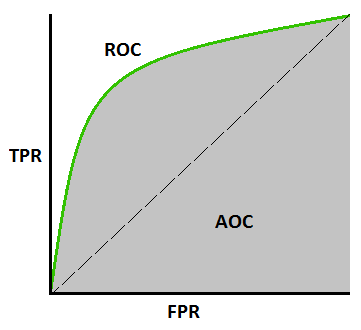
\includegraphics[width=0.5\linewidth]{images/rocauc.png}
    \label{fig:rocauc}
\end{figure}

\subsection{Model Validation and Evaluation}

The verified reviews in the Amazon Product Review dataset represent individuals who bought or used the item and paid a price available to most shoppers. Initially, we believed that a verified review may be more credible than an unverified one, and thus may affect the model. In order to see if whether or not this belief was true, tests were conducted with and without including the column in modeling. See Table \ref{tab:svm-prelim}. To summarize the results, it seems to change some metrics by less than a percent. As a result, we decided that the verified column is not significant enough and excluded it from most modeling steps.

\subsubsection{Logistic Regression}
Models were created for the following: baseline data, preprocessed data, stemmed data, and lemmatized data; each set of 4 was vectorized by either the CountVectorizer() or TfidfVectorizer(), resulting in a total of 8 sets of data. Initial tests were done with the default parameters for Logistic Regression, trained on the training data and tested on the validation data, resulting in the following classification reports found in Figure \ref{fig:logreg_base}, with the CountVectorized data on the left and the TfidfVectorized data on the right. Across all baseline tests, the results in terms of precision, recall, F1 score, and accuracy are similar. This should come as no surprise considering despite going through preprocessing, the baseline data is still quite similar with the 3 preprocessed datasets. From this baseline test, the best performing model is the baseline Tfidf model, with a macro average F1 score of 0.73 and an overall accuracy of 0.93.

\begin{figure}[!htb]
    \centering
    \caption{Logistic Regression Baseline}
    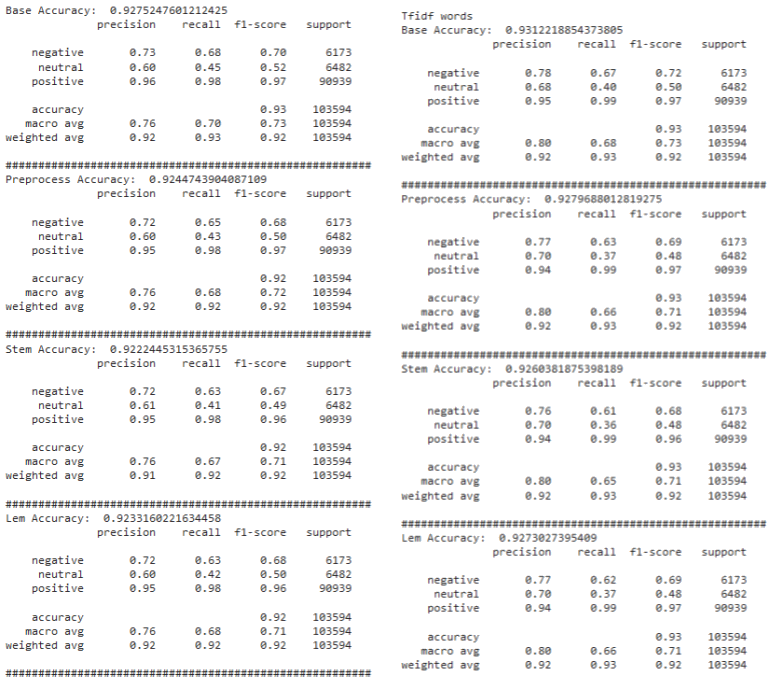
\includegraphics[width=0.9\linewidth]{images/logreg_baseline_light.png}
    \label{fig:logreg_base}
\end{figure}

The baseline results seem promising, but hyperparameter tuning was performed on the validation data in an attempt to improve them. To save on computation time and cost, a RandomizedSearchCV with 3 cross validations and 20 iterations was utilized. The parameters that were tuned were the C value, which is the inverse of regularization strength, and the solver type. Out of the many parameters that Logistic Regression has access to, only these two were selected to be tuned due to the following reasons: 1. Many of the parameters are solver specific, meaning many fits will fail due to incompatibility and 2. Only 4 of the 6 solvers support multinomial Logistic Regression. The resulting parameter grid is as follows: [{'C':[0.001, 0.01, 0.1, 1, 10, 100], `solver':['lbfgs', `newton-cg', `sag', `saga']}]. The best parameters from each of the 8 models were taken and then fed into their final models that trained on the training data and tested with the test data. Similar to the baseline test, the overall best performing model was the baseline TfidfVectorized data with a C value of 1 and a sag solver. The results, however, are roughly the same with extremely slight improvements. More specifically, the macro average F1 Score stayed around the same, but the overall accuracy increased by less than a percent, going from 0.9312 for the baseline to 0.9315 for the tuned model. The results for all models can be seen in Figure \ref{fig:logreg_final}.

\begin{figure}[!htb]
    \centering
    \caption{Logistic Regression After Hypertuning}
    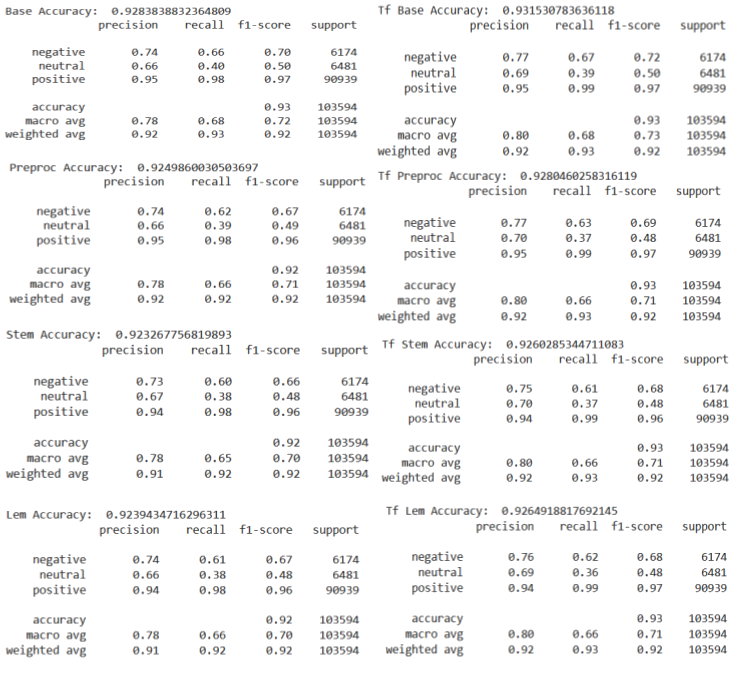
\includegraphics[width=0.9\linewidth]{images/logreg_final_light.png}
    \label{fig:logreg_final}
\end{figure}

For the best performing model (baseline Tfidf), a ROC AUC Curve was created, showing the micro and macro average ROC AUC Score, as well as individual scores for the positive, neutral, and negative classes. For this model, the micro average ROC AUC Score was 0.99, the macro average score is 0.96, the negative class score is 0.98, the neutral class score is 0.94, and the positive class score is 0.97.  Pictured in Figure \ref{fig:logregcurve} is the ROC AUC Curve.
\begin{figure}[!htb]
    \centering
    \caption{Logistic Regression ROC AUC Curve}
    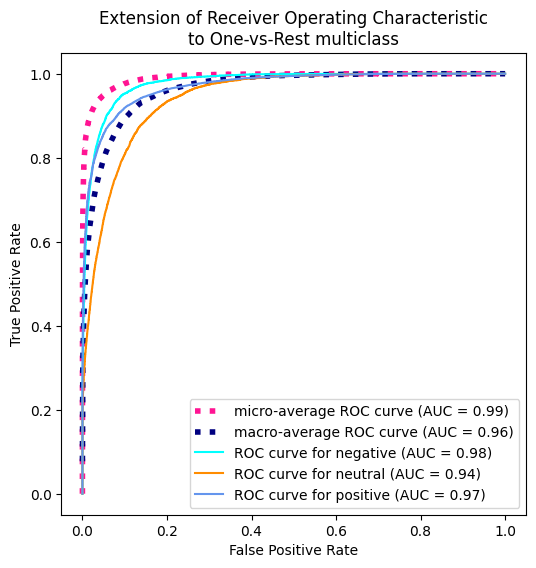
\includegraphics[width=0.5\linewidth]{images/logreg_roccurve.png}
    \label{fig:logregcurve}
\end{figure}


One important thing to note is the time it took for training. For each of the CountVectorizer() tests, it took approximately 1 hour and 50 minutes for each RandomizedSearchCV(), and around 20 to 30 minutes for training the final model. On the other hand, the TfidfVectorizer() tests took only around 10 to 20 minutes for RandomizedSearchCV() and roughly 2 to 3 minutes for training. Due to this, even though all of the results are fairly similar, we can say with certainty that the TfidfVectorizer() data performed the best.

\subsubsection{SVM}
To test the effectiveness of support vector machines, we ran through 2 notebooks. The goal of the first notebook is to find which \textit{baseline} SVC model performs best on which configurations of the dataset. The first of the different configurations tested was which column to use of the columns listed in Figure \ref{fig:transform-cols}. The next configuration tested was which preprocessing method was best, as can be seen in Figure \ref{fig:preprocessed-data}. The final difference tested was which vectorizer performed best, either BoW or TF-IDF. Since there are many configurations, this performed on a small subset of the full data using default parameters of SciKit-Learn's SVC classifier. The performance was tested on the basis of accuracy, F1 Score, Precision, and ROC AUC score. See Table \ref{tab:svm-prelim}.

\begin{table}[!htb]
    \centering

    \caption{SVM Preliminary results}
    \scalebox{0.75}{
\begin{tabular}{llrrrrrrrr}
\hline
 &  & \multicolumn{2}{r}{Accuracy} & \multicolumn{2}{r}{F1 Score} & \multicolumn{2}{r}{Precision} & \multicolumn{2}{r}{ROC AUC} \\
 & Vectorizer & BoW & TF-IDF & BoW & TF-IDF & BoW & TF-IDF & BoW & TF-IDF \\
Columns & Preprocessing &  &  &  &  &  &  &  &  \\
\hline
\multirow[t]{4}{*}{reviewText} & None & 0.881 & 0.884 & 0.826 & 0.834 & 0.895 & 0.884 & 0.852 & 0.888 \\
 & Baseline & 0.882 & 0.883 & 0.828 & 0.832 & 0.896 & 0.890 & 0.835 & 0.864 \\
 & Lemmatized & 0.881 & 0.883 & 0.827 & 0.832 & 0.895 & 0.891 & 0.831 & 0.862 \\
 & Stemmed & 0.882 & 0.885 & 0.830 & 0.836 & 0.881 & 0.827 & 0.834 & 0.861 \\
\cline{1-10}
\multirow[t]{4}{*}{reviewText, verified} & None & 0.881 & 0.884 & 0.826 & 0.833 & 0.895 & 0.827 & 0.852 & 0.885 \\
 & Baseline & 0.882 & 0.883 & 0.828 & 0.832 & 0.896 & 0.865 & 0.836 & 0.862 \\
 & Lemmatized & 0.881 & 0.882 & 0.827 & 0.831 & 0.895 & 0.858 & 0.831 & 0.860 \\
 & Stemmed & 0.882 & 0.883 & 0.830 & 0.834 & 0.881 & 0.853 & 0.834 & 0.859 \\
\cline{1-10}
\multirow[t]{4}{*}{reviewTextWithSummary} & None & 0.905 & \textbf{0.908} & 0.877 & \textbf{0.883} & 0.903 & \textbf{0.907} & 0.925 & \textbf{0.941} \\
 & Baseline & 0.906 & 0.906 & 0.880 & 0.879 & 0.907 & 0.907 & 0.913 & 0.924 \\
 & Lemmatized & 0.906 & 0.903 & 0.880 & 0.876 & 0.907 & 0.901 & 0.910 & 0.923 \\
 & Stemmed & 0.907 & 0.905 & 0.882 & 0.878 & 0.906 & 0.901 & 0.912 & 0.925 \\
\cline{1-10}
\multirow[t]{4}{*}{reviewTextWithSummary, verified} & None & 0.904 & 0.907 & 0.877 & 0.882 & 0.902 & 0.906 & 0.925 & 0.939 \\
 & Baseline & 0.906 & 0.905 & 0.881 & 0.879 & 0.907 & 0.907 & 0.913 & 0.922 \\
 & Lemmatized & 0.906 & 0.904 & 0.880 & 0.877 & 0.907 & 0.905 & 0.910 & 0.921 \\
 & Stemmed & 0.907 & 0.905 & 0.882 & 0.879 & 0.906 & 0.904 & 0.912 & 0.924 \\
\cline{1-10}
\hline
\end{tabular}
    }

    \label{tab:svm-prelim}
\end{table}

Based on the results of Table \ref{tab:svm-prelim}, we can see that not including the summary is always worse, TF-IDF generally performs well, and including the verified column does not improve the result in any meaningful way. There is a fair representation of the different preprocessing types in the top scores. Therefore the full testing of SVM can be done on the 4 preprocessing types on the `reviewTextWithSummary' column using TF-IDF vectorization.

The second notebook tests these configs following the flowchart in Figure \ref{fig:model-arch}. This notebook was run on the full, nearly 700,000, entry dataset. In order to run this in a timely manner, we used Google Colab using the `cuML' SVC classifier. The baseline performance can be seen in Table \ref{tab:svm-baseline}. Once the baseline was found, we performed hyperparameter tuning on each model. The best parameters for each of these tests were the same, i.e. set the kernel to `RBF', the $C$ value to 10, and the gamma to `scale'. The result of the hyperparamater tuned models on the test set can be seen in Table \ref{tab:svm-final}. The F1 Scores and precision scores show the weighted average, the ROC AUC score is calculated based on `one vs rest', and the Grid score is based on the `best\_score\_' from the hyperparameter tuning. 

\begin{table}[!htb]
    \centering
    \caption{Baseline SVM results on validation set}

    \begin{tabular}{lrrr}
    \hline
    Preprocessing & F1 score & Accuracy & Precision \\
    \hline
    None & 0.928 & 0.936 & 0.930 \\
    Baseline & 0.922 & 0.932 & 0.926 \\
    Stemmed & 0.920 & 0.930 & 0.924 \\
    Lemmatized & 0.921 & 0.931 & 0.925 \\
    \hline
    \end{tabular}

    \label{tab:svm-baseline}
\end{table}


\begin{table}[!htb]
    \centering
    \caption{Hyperparameter tuned SVM results on testing set}

    \begin{tabular}{lrrrrr}
    \hline
    Preprocessing & Grid Score & F1 Score & Accuracy & Precision & ROC AUC \\
    \hline
    None & 0.927 & 0.933 & 0.939 & 0.932 & 0.918 \\
    Baseline & 0.923 & 0.927 & 0.935 & 0.928 & 0.898 \\
    Stemmed & 0.923 & 0.925 & 0.934 & 0.926 & 0.895 \\
    Lemmatized & 0.923 & 0.926 & 0.934 & 0.927 & 0.895 \\
    \hline
    \end{tabular}


    \label{tab:svm-final}
\end{table}

Based on these result it can be seen that the best performing model is the one without any text preprocessing. The ROC curve for this model can be seen in Figure \ref{fig:svm-roc}.

\begin{figure}[!htb]
    \centering
    \caption{SVM best model ROC Curve}
    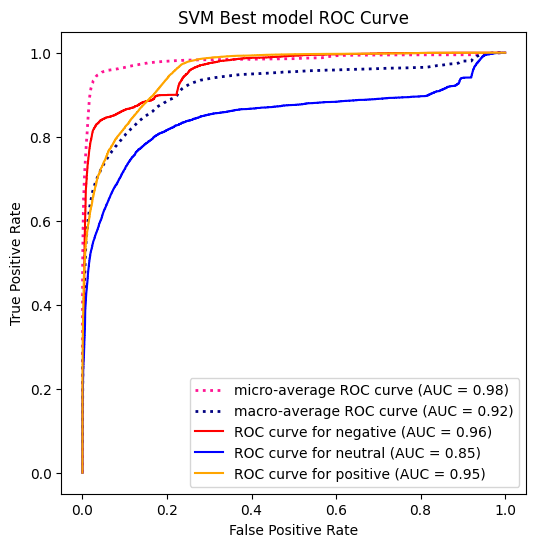
\includegraphics[width=0.5\linewidth]{images/svm/svm-final-roc.png}
    \label{fig:svm-roc}
\end{figure}

\subsubsection{Naive Bayes}
There were 4 different models that were created for Naive Bayes (NB), with all of them being variants and different types under the NB classifier. The models tested were: Gaussian NB, Bernoulli NB, Complement NB, Multinomial NB. The process for each of the four models involved dividing the dataset into training, validation, and testing sets, allocated at 70\%, 15\%, 15\% percent respectively. These percentages ensured that the model trained under one subset, fine-tuning with hyperparameters on the next step, and evaluated the separate subset on unseen data or the testing set. The target variable labelled `Overall' was utilized for all models, while the data features served as predictors for model prediction. The only exception was the Bernoulli classifier, which required the target variable `Sentiment' due to its binary type. 

It is important to note a limitation in the data preprocessing step. First, English stopwords from the NLTK package `stopwords' found common words such as ``the'', ``is'', ``and'' were removed from text during natural language processing tasks due to the insignificant weight each word held. Lematizing was also used to reduce words to base forms. Regular expressions removed digits from the text and non-words for consistency with text analysis. After doing this, TfidVectorizer was used to convert text documents into a matrix of TF-IDF features. Due to spacing in the hardware, this process of getting the max features took significant time. As a result, the maximum number of features was set to 2000 for words. This result was due to the combination of limitation in hardware and the dataset being very large. If further analysis were conducted with higher maximum features, the accuracy could be better. 

After processing words, several models were created, and each model included a baseline version, which aimed to access the initial performance before the hyperparameter fine-tuning step. A classification report was created to show the accuracy for each models, which are referred below: 

\begin{figure}[!htb]
    \centering
    \caption{Classification Report for Gaussian NB Baseline}
    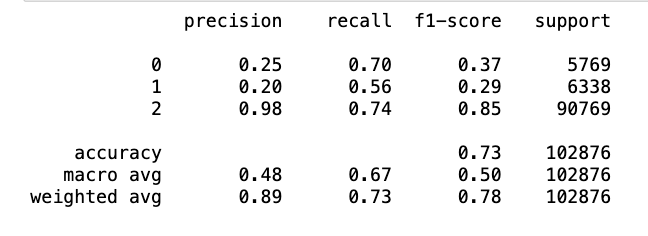
\includegraphics[width=0.39\linewidth]{images/Gau1.png}
    \label{fig:Gaussian NB Baseline}
\end{figure}
\begin{figure}[!htb]
    \centering
    \caption{Classification Report for Multinomial NB Baseline}
    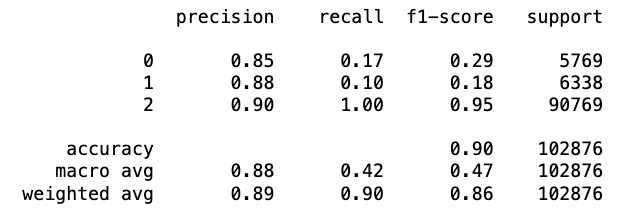
\includegraphics[width=0.39\linewidth]{images/Multi1.png}
    \label{fig:Multinomial NB Baseline}
\end{figure}
\begin{figure}[!htb]
    \centering
    \caption{Classification Report for Bernoulli NB Baseline}
    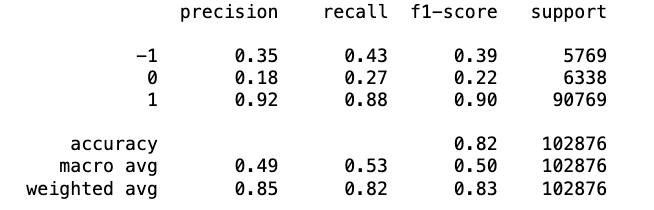
\includegraphics[width=0.39\linewidth]{images/Bern1.png}
    \label{fig:Bernoulli NB Baseline}
\end{figure}
\begin{figure}[!htb]
    \centering
    \caption{Classification Report for Complement NB Baseline}
    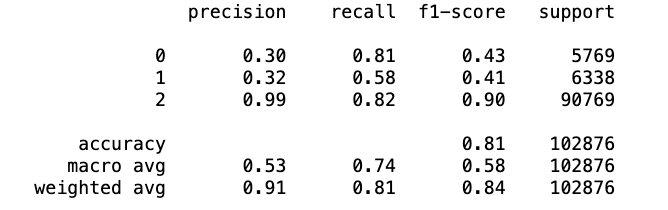
\includegraphics[width=0.39\linewidth]{images/Comp1.png}
    \label{fig:Complement NB Baseline}
\end{figure}
In summary the accuracy of baseline for Gaussian, Multinomial, Bernoulli, and Complement were respectively: 0.73, 0.90, 0.82, 0.81. The classifiers were first initialized based on the assumptions of the features for each specific model. They were then trained to find patterns within features and labels. In the post-training, the classifiers predicted outcomes on the test data. 

In all models, fine-tuning was conducted to refine the baseline performance. This involved creating a hyperparamter grid, which signaled a range of hyperparameters for tuning. The grid used various parameters, each specific to the type of NB model. The final model was constructed using the best hyperparameters from the grid and trained using the training set to predict outcomes on the testing set. This report utilized each model's classification report to calculate the precision, recall, F1-score, and support for each class.  Below are the results for the best hyperparameters for each model: 

\begin{figure}[!htb]
    \centering
    \caption{Classification Report for Gaussian NB Best Parameters}
    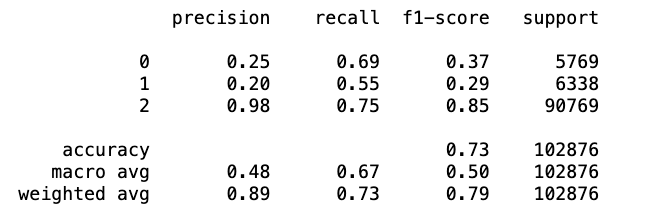
\includegraphics[width=0.39\linewidth]{images/Gau2.png}
    \label{fig:Gaussian NB Best Parameters}
\end{figure}
\begin{figure}[!htb]
    \centering
    \caption{Classification Report for Multinomial NB Best Parameters}
    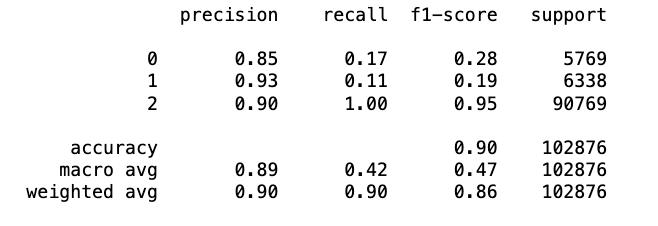
\includegraphics[width=0.39\linewidth]{images/Multi2.png}
    \label{fig:Multinomial NB Best Parameters}
\end{figure}
\begin{figure}[!htb]
    \centering
    \caption{Classification Report for Bernoulli NB Best Parameters}
    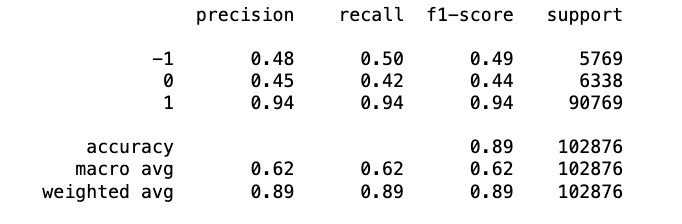
\includegraphics[width=0.39\linewidth]{images/Bern2.png}
    \label{fig:Bernoulli NB Best Parameters}
\end{figure}
\begin{figure}[!htb]
    \centering
    \caption{Classification Report for Complement NB Best Parameters}
    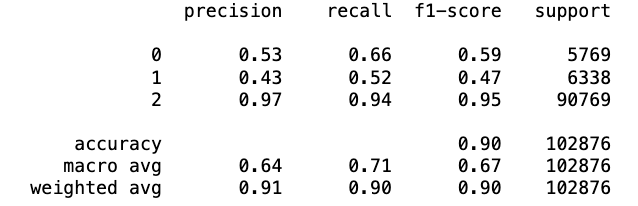
\includegraphics[width=0.39\linewidth]{images/Comp2.png}
    \label{fig:Complement NB Best Parameters}
\end{figure}
In summary the accuracy of best parameters for Gaussian, Multinomial, Bernoulli, and Complement were respectively: 0.73, 0.90, 0.89, 0.90. The macro average are respectively: 0.5, 0.47, 0.62, 0.67. The weighted average are respectively: 0.79, 0.86, 0.89, 0.90. It can be seen that Complement had the higher values in each case.

Gaussian and Multinomial remained the current accuracy, but Bernoulli and Complement each increased its accuracy. In terms of best parameter, Gaussian NB had parameters for `prior' which specified the prior probabilities of the classes and in this model case, were three sets in None, distribution in [0.2, 0.8], and distribution in [0.5, 0.5]. These are set as an example for the model to run. The `var\_smoothing' specified the largest variance of all features for stability. In this model case, it was provided with 1e-9, 1e-8, 1e-7, and 1e-6. In the Multinomial parameters, the `alpha' hyperparameter controlled the Laplace smoothing for the classifier and were tested with values of [0.0001, 0.001, 0.01, 0.1, 1, 10]. The `force\_alpha' parameter of [True, False] specified whether the algorithmn should force alpha to be positive or not with True being positive. The `fit\_prior' also had values of [True, False] and showed if class probabilities were st prior. For Bernoulli, the parameters were `alpha', `binarize', `fit\_prior', and `class\_prior'. All parameters were previously mentioned, with the `binarize' showing the threshold value for binarizing features if the input data was not already binary set at values of [0.0, 0.1, 0.2]. The Complement NB used parameters `alpha', `fit\_prior', and `norm', with norm being if a second normalization of the weights was performed.

After this step, an ROC-AUC curve was made for the best model of Complement Naive Bayes. This model was chosen because it had the highest average macro average at 0.9, highest weighted average at 0.67, and tied for the highest accuracy at 0.9. The result of the ROC-AUC curve is shown:
\begin{figure}[!htb]
    \centering
    \caption{Complement NB ROC}
    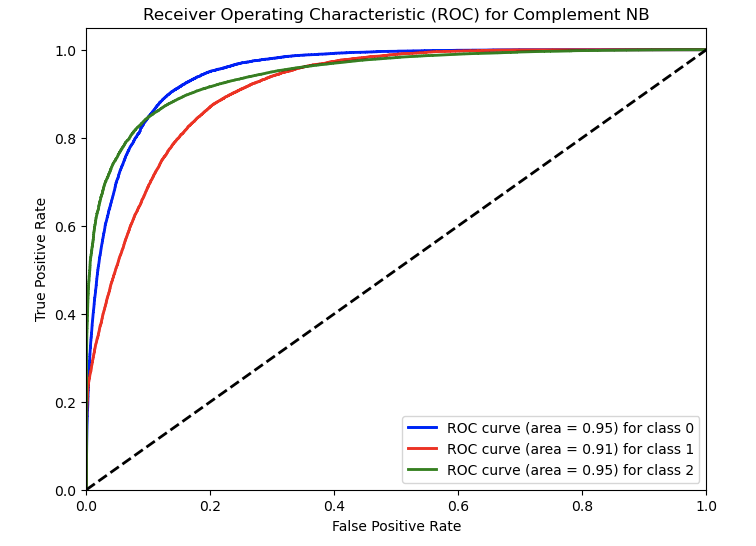
\includegraphics[width=0.39\linewidth]{images/ROC2.png}
    \label{fig:NB ROC}
\end{figure}

It can be inferred that the ROC curve under this model showed high true positivity rate for each of the classes of 0, 1, 2. The areas under each are all above 0.91, which is generally acceptable for a model that performs well in distinguishing between the classes. 


\subsubsection{XGBoost}
To test XGBoost, we went through a set of different tests and methods to achieve some feasible results. Since this model is intense in memory usage, we stuck to using only a TfidfVectorizer to obtain results quicker. After preprocessing the data and cleaning up the stopwords, we performed lemmatization on the entire dataset. The output was then put through the TfidfVectorizer for the vectorization. We started by attempting to train the model on this sparse set of data output from TFidfVectorizer. To try improving the results, we attempted to perform hyper-parameter tuning using RandomizedSearchCV on a set of possible combinations. However, that did not deliver feasible results during the training process. We attempted to use GridSearchCV on a simpler set of parameters to try improving the model's performance on the sparse data. Since XGBoost is a memory intensive model and GridSearchCV performs exhastive search when trying every possible combination, we used a different machine with better hardware capability. The results, however, still did not improve substantially.

Several tests were performed on the sparse data without preprocessing, with preprocessing, with stemming, and with lemmatization. We applied each possible scenario on a baseline model and on a version that is assumed to be tuned using the parameters that were obtained from the GridSearchCV. The results for the majority of the tests on the sparse data were relatively poor.
\begin{figure}[!htb]
    \centering
    \caption{Baseline sparse test results}
    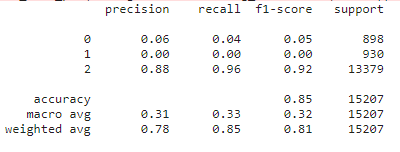
\includegraphics[width=0.5\linewidth]{base_mod_spars.png}
    \label{fig:base_mos_spars}
\end{figure}

Figure \ref{fig:base_mos_spars} references results one of the test cases on the baseline model with sparse data.

\begin{figure}[!htb]
    \centering
    \caption{Tuned sparse test results}
    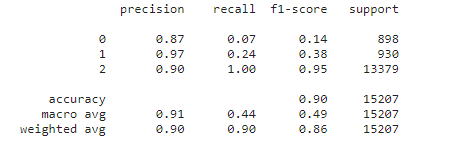
\includegraphics[width=0.5\linewidth]{Tuned_mod_spars.png}
    \label{fig:Tuned_mod_spars}
\end{figure}

Figure \ref{fig:Tuned_mod_spars} represents the results of a test case on a tuned model with the the sparse data. While the results improved a little, they are still not in good standing. 

XGBoost is  known for not working well on sparse data. To overcome this, we utilized tools available to us from scipy that allowed us to make the data more dense. A more dense dataset means that it would take up more disk space and use more memory in processing. Increasing the density of the entire dataset was not possible due to hardware complications with memory. We had to substantially resample the data and ended up being able to increase the density of only fifteen percent of the data without any hardware complications. 

Using the dense version, we repeated the same test cases training the model on unpreprocessed, preprocessed, stemmed, and lemmatized versions of the data. The overall results improved by a lot. 
\begin{figure}[!htb]
    \centering
    \caption{Sample dense test result}
    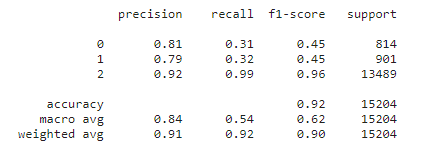
\includegraphics[width=0.5\linewidth]{dense_result_snippit.png}
    \label{fig:dense_result_snippit}
\end{figure}

Based on the results in \ref{fig:dense_result_snippit}, we can tell the overall results for each category is improved. The precision, recall, and f1-scores for negative and neutral sentiment are substantially better compared to the results of the sparse data from \ref{fig:base_mos_spars} and \ref{fig:Tuned_mod_spars}. 

\begin{figure}[!htb]
    \centering
    \caption{Results of the best Model}
    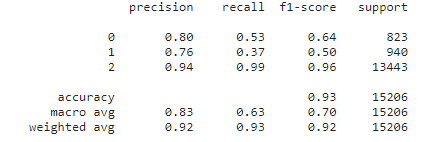
\includegraphics[width=0.5\linewidth]{Best_model.png}
    \label{fig:Best-model}
\end{figure}

The results from \ref{fig:Best-model} indicate the performance of the best XGBoost model for all the tests. The best results came from a baseline version of the model that trained on data that was not preprocessed. The overall accuracy of this model is around 93 percent. The precision, recall and f1-scores are also relatively higher compared to other test cases for the dense data or compared to any of the sparse data. While in this case the preprocessing nor tuning of results really improved the results much, the fairly high and efficient results obtained just from the baseline model on data that wasn't even preprocessed shows how XGBoost is capable of performing really well. 
\begin{figure}[!htb]
    \centering
    \caption{ROC Curve for best XGBoost model}
    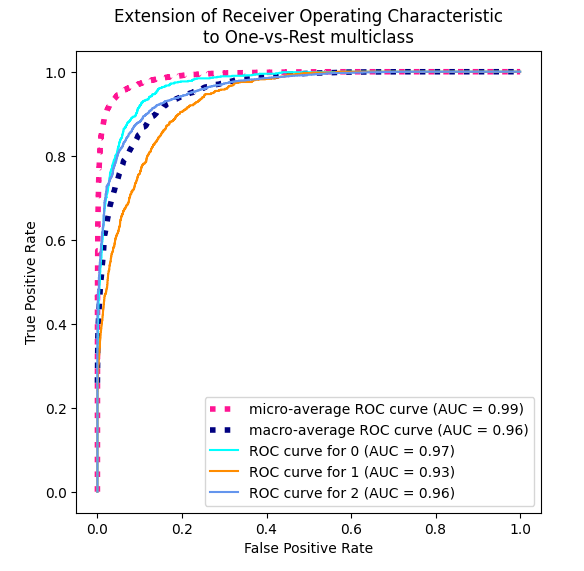
\includegraphics[width=0.5\linewidth]{ROC_curve_XGBoost.png}
    \label{fig:ROC-curve-XGBoost}
\end{figure}
There was some minor variation in the ROC result depending on the sentiment indicated in \ref{fig:ROC-curve-XGBoost} . The results were relatively skewed to the right. However, the results were relatively high. The overall macro-average comes out to be about 96 percent.

\subsubsection{Comparison Model Performance}

The macro average F1 score for each implementation's best model is listed in Table \ref{tab:final-compare}.

\begin{table}[!htb]
    \centering
    \caption{Best Model Performance Comparison}
    \begin{tabular}{cc}
    \hline
        Model & Macro Average F1 Score\\
    \hline
        Logistic Regression & 0.73\\
        SVM & \textbf{0.76}\\
        Naive Bayes & 0.67\\
        XGBoost & 0.70\\
    \hline
    \end{tabular}
    \label{tab:final-compare}
\end{table}

The overall best model was SVM using the TF-IDF vectorizer on the `reviewWithSummaryText' without any preprocessing applied to it. This was due to the fact that training SVM used an exhaustive search in both preliminary testing with dataset and preprocessing and final testing with hyperparameter tuning. It should also be noted that for the final testing, the Google Colab A100 GPU was used for training.

The results for each of the models, however, could be improved on. 

In the case for Logistic Regression, RandomizedSearchCV() was used to save on computation time and cost. As a result, the hyperparameter tuning step was likely not the most optimal. A more exhaustive search using additional parameters, higher CVs, and number of iterations could have been used. Alternatively, a GridSearchCV() could have been performed. 

In the context of Naive Bayes, where the TF-IDF vectorizer utilized only 2000 features, there exists an opportunity of refinement and optimization to better represent the data. The decision to limit the feature set to 2000 features was driven by computational constraints and the exploration of the dataset's complexity. Further investigation and fine-tuning would ensure selected features adequately capture the full dataset. Given the many features in the dataset, a selection of 2000 features may not fully capture the entire data. In addition, other types of Naive Bayes models can be used, such as Categorical NB, to compete with the best model of Complement NB.

For XGBoost, the main limiting factor was the hardware. Due to having to convert to dense data, the machine would often run out of memory when modeling, resulting in the use of a subset of the data. If we had better hardware, then a more exhaustive hyperparameter list could have been used to perform hyperparameter tuning using RandomizedSearchCV or GridSearchCV leading to a more optimal result.

\subsubsection{Conclusion}

Ultimately, the evolution of online shopping within society has led to the importance of consumer reviews as an influential factor in purchasing decisions and market trends. In many available platforms, Amazon has emerged as a leading source for consumer feedback for many and diverse categories of products. Using sentiment analysis techniques and machine learning models, organizations can use insights gained from this research to gauge customer satisfaction and identify areas for improvement. Based on our research, the overall best performing model was SVM.

One issue with the preprocessing step found late into the modeling step was the removal of stopwords. Stopwords are a set of commonly used words such as "a" and "the". However, after analyzing the stopword list, it also includes words that are heavy in context such as "don't." This created the problem of changing the meaning of certain reviews. For example, if a negative review saying "don't buy this product" went through preprocessing, then removing the stopwords would change this to "buy product," which completely changes its meaning and likely hurts the model. Based on the results, there are not many entries that are affected by this, but there are some nonetheless. Additionally, the stemming and lemmatization steps were only performed on the preprocessed data, which could have attributed to their accuracy being lower than the unprocessed data.

In the future, we can improve the project overall by incorporating more reviews from the original dataset, instead of only the categories mentioned in Table \ref{tab:amazon-categories}. Though our project is focused on categorizing reviews, we can also train on non review data to teach the models the variations in human written text. Finally, we can potentially combine the models in a majority voting ensemble model to overcome any shortcomings in each of the models.

\printbibliography

\appendix
\section{Project management charts}
\begin{figure}[!htb]
    \centering
    \caption{Pert Chart}
    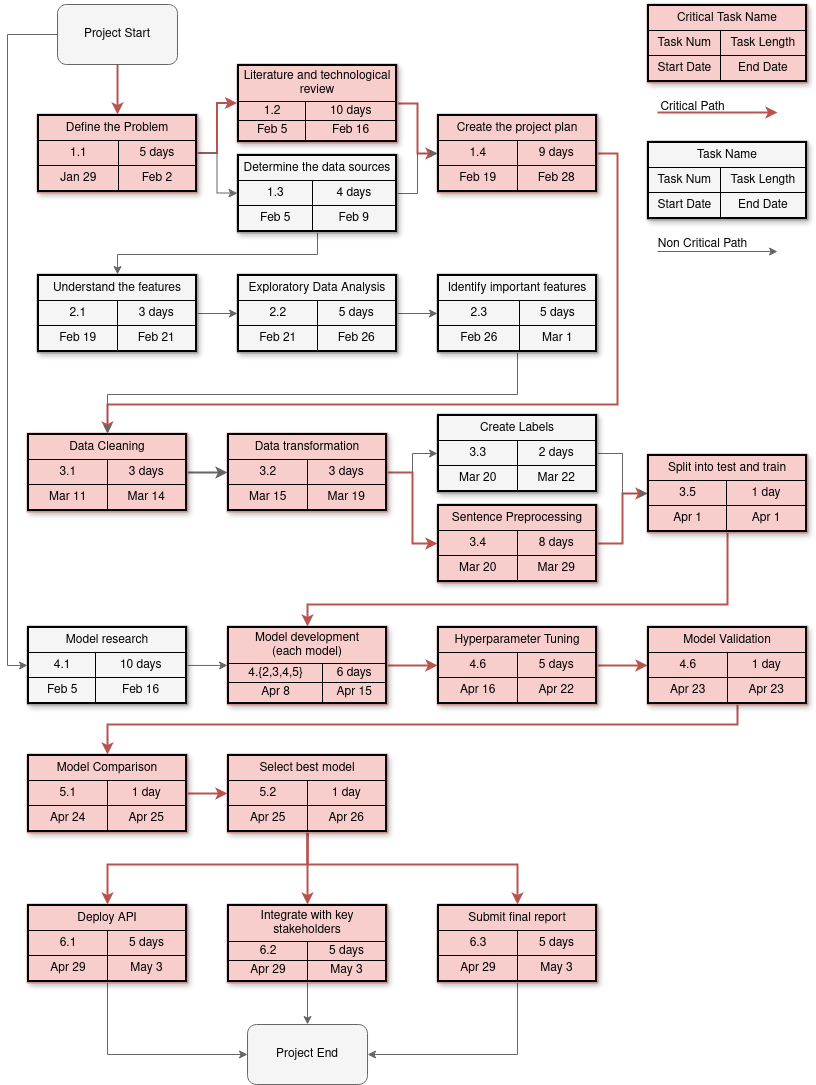
\includegraphics[height=0.75\textheight]{images/Pert.png}
    \label{app:fig:pert}
\end{figure}

\begin{figure}[!htb]
    \centering
    \caption{Gantt Chart}
    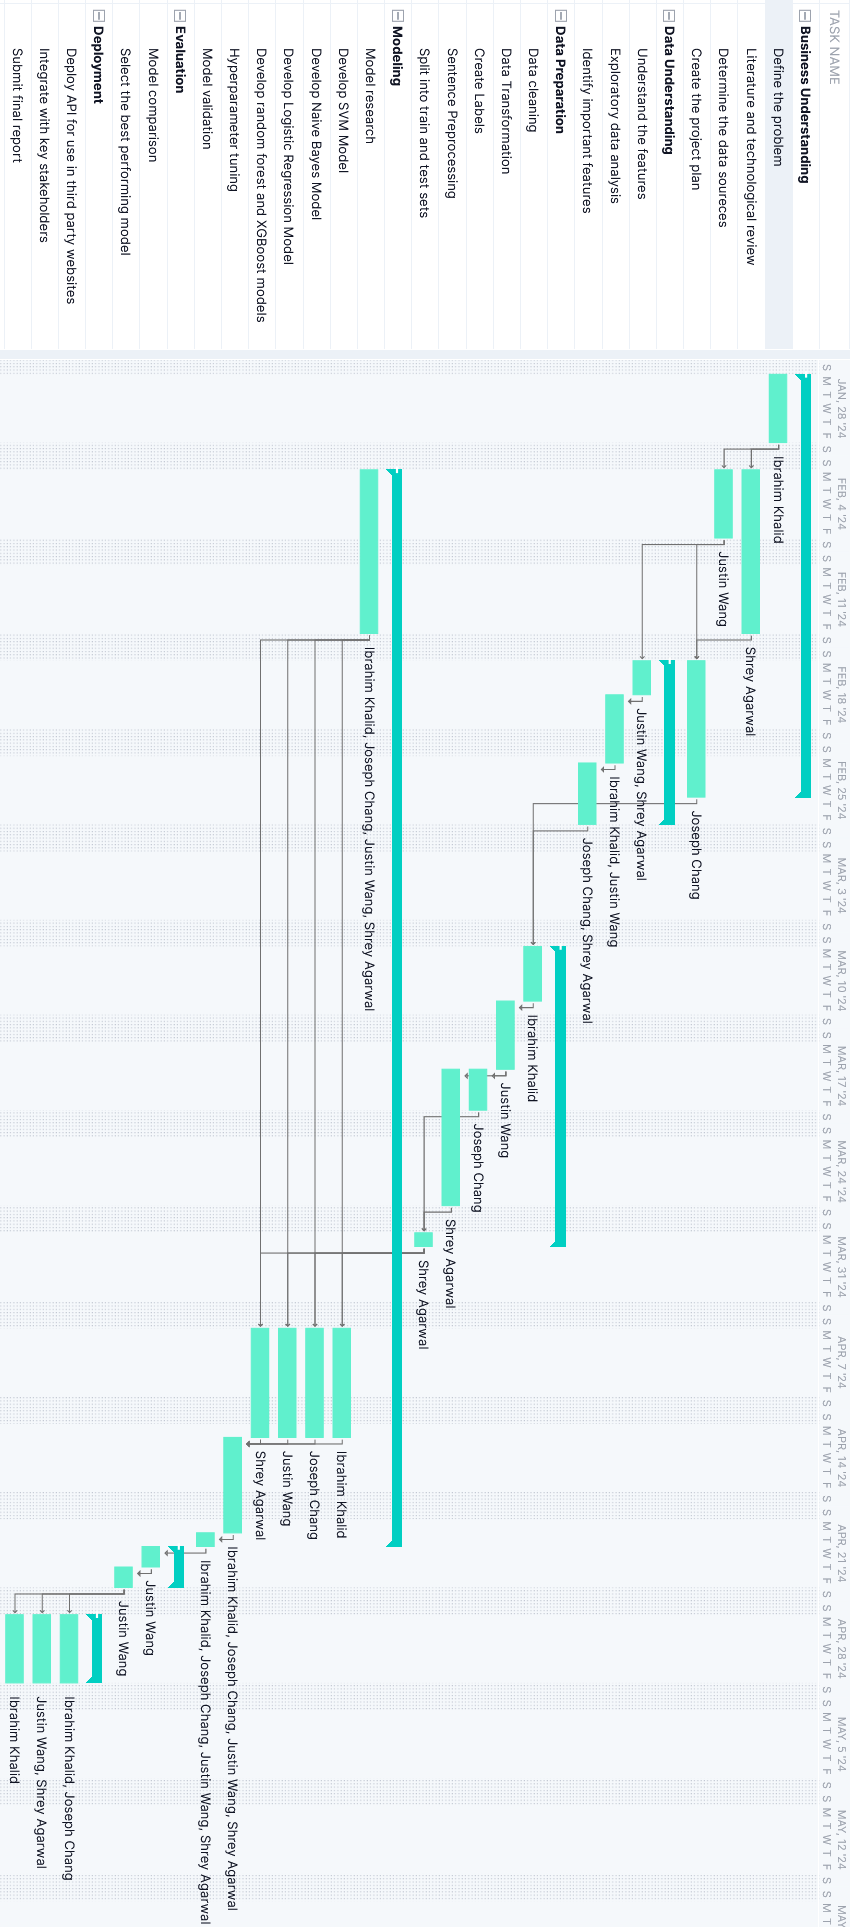
\includegraphics[height=0.85\textheight]{images/Gantt_rotated.png}
    \label{app:fig:gantt}
\end{figure}

\section{Dataset}

\begin{figure}
    \centering
    \caption{Preprocessed Datasets: first 5 rows}
    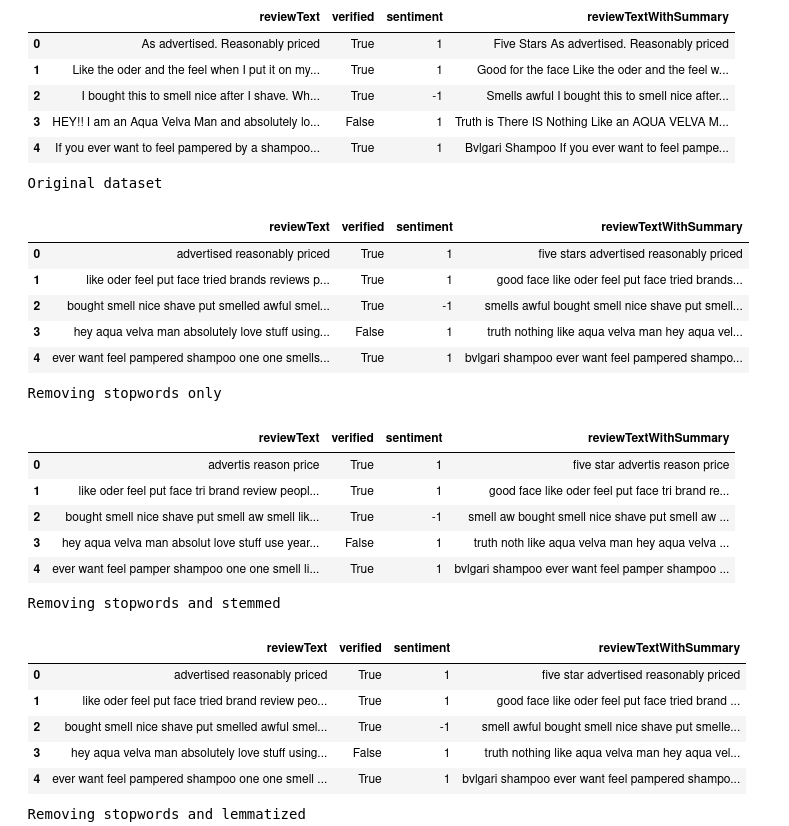
\includegraphics[width=0.9\linewidth]{images/preprocessing-compare.png}
    \label{fig:preprocessed-data}
\end{figure}

\begin{figure}
    \centering
    \caption{Baseline preprocessing WordCloud without summary}
    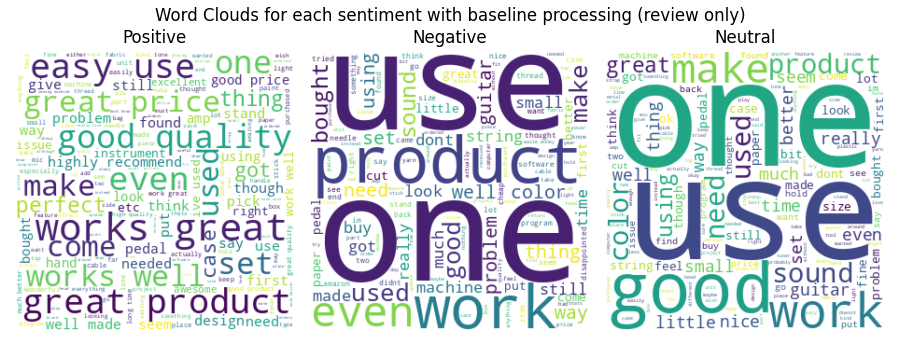
\includegraphics[width=\linewidth]{images/results/Word_Clouds_for_each_sentiment_with_baseline_processing_(review_only).png}
    \label{fig:wordcloud-baseline}
\end{figure}

\begin{figure}
    \centering
    \caption{Baseline preprocessing WordCloud with summary}
    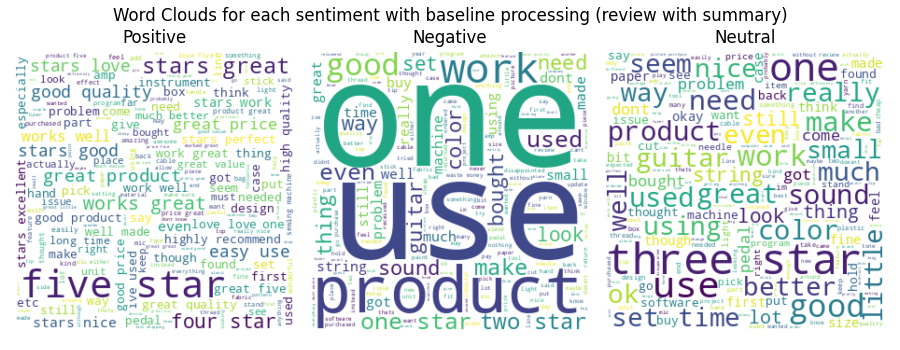
\includegraphics[width=\linewidth]{images/results/Word_Clouds_for_each_sentiment_with_baseline_processing_(review_with_summary).png}
    \label{fig:wordcloud-summary}
\end{figure}

\begin{figure}
    \centering
    \caption{Top 10 word counts with and without summary}
    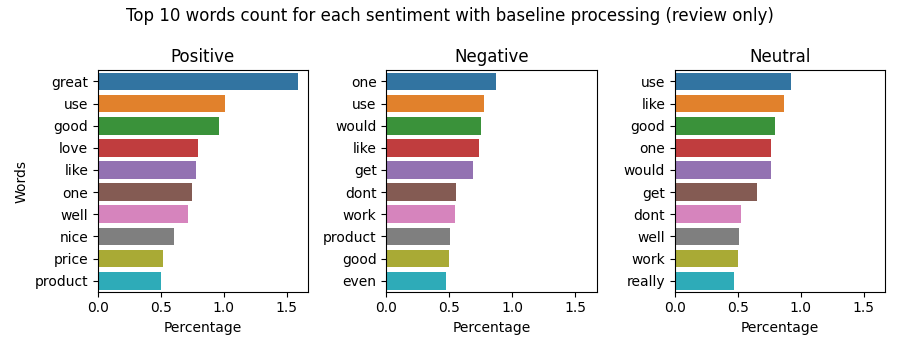
\includegraphics[width=0.9\textwidth]{images/results/Top_10_words_count_for_each_sentiment_with_baseline_processing_(review_only).png}
    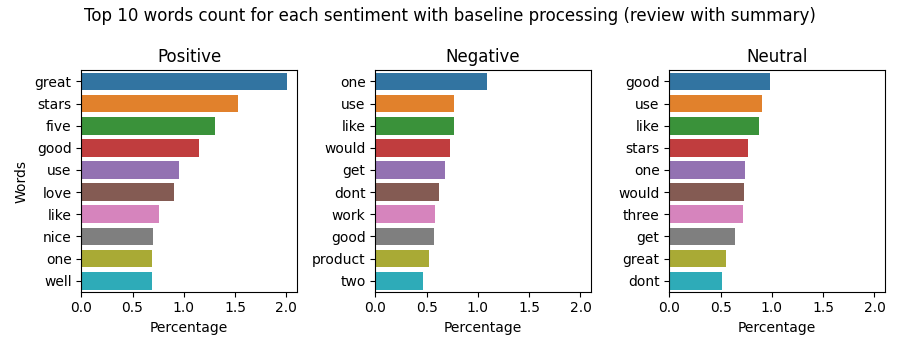
\includegraphics[width=0.9\textwidth]{images/results/Top_10_words_count_for_each_sentiment_with_baseline_processing_(review_with_summary).png}
    \label{fig:top-10-barplot}
\end{figure}


\end{document}